% ==============================================================================
% CHƯƠNG 3: CÀI ĐẶT VÀ THỰC NGHIỆM CHƯƠNG TRÌNH
% ==============================================================================
\chapter{CÀI ĐẶT VÀ THỰC NGHIỆM CHƯƠNG TRÌNH}
\label{chap:cai_dat_thuc_nghiem}

\section{Cài đặt môi trường và kịch bản khởi tạo}
\label{sec:cai_dat_moi_truong}

\subsection{Cấu hình môi trường phát triển và thực thi}
Hệ thống POS Quản lý bán hàng được thiết kế theo kiến trúc Micro-services/Monorepo phân tách rõ ràng giữa máy chủ Back-end và giao diện Front-end. Môi trường yêu cầu chuẩn để triển khai ứng dụng bao gồm:
\begin{itemize}[leftmargin=1.5cm]
    \item \textbf{Môi trường máy chủ Back-end:} Java Development Kit phiên bản OpenJDK 25, Apache Maven 3.9+, Spring Boot 4.1.0.
    \item \textbf{Môi trường giao diện Front-end:} Node.js phiên bản 20.x trở lên, trình quản lý gói NPM 10.x, Vite 8 và React 19.
    \item \textbf{Hệ quản trị cơ sở dữ liệu:} MySQL Server phiên bản 8.0, cấu hình bảng mã ký tự \texttt{utf8mb4} và đối chiếu \texttt{utf8mb4\_unicode\_ci}.
    \item \textbf{Hạ tầng Container hóa:} Docker Engine phiên bản 24.x trở lên và Docker Compose v2.
\end{itemize}

\subsection{Cấu hình biến môi trường và thông số ứng dụng}
Để đảm bảo an toàn thông tin theo nguyên tắc chuẩn của các dự án mã nguồn mở, toàn bộ các thông tin nhạy cảm (như mật khẩu cơ sở dữ liệu, khóa bí mật JWT, khóa xác thực AWS S3 và PayOS) đều được tách biệt hoàn toàn khỏi mã nguồn và nạp động thông qua các biến môi trường (\texttt{.env}).

\subsubsection{Cấu hình máy chủ Back-end (\texttt{application.properties})}
Đoạn trích cấu hình trung tâm của Spring Boot tại tệp \texttt{billingsoftware/src/main/resources/application.properties}:
\begin{lstlisting}[language=sh, caption={Cấu hình thông số hệ thống trong application.properties}]
spring.application.name=billingsoftware
server.servlet.context-path=/api/v1.0

# Cau hinh ket noi MySQL voi ky tu UTF-8 va timezone UTC
spring.datasource.url=jdbc:mysql://${DB_HOST}:${DB_PORT}/${DB_NAME}?useSSL=false&serverTimezone=UTC&allowPublicKeyRetrieval=true
spring.datasource.username=${DB_USER}
spring.datasource.password=${DB_PASS}

# Che do kiem tra nghiem ngat schema va kich hoat Flyway
spring.jpa.database-platform=org.hibernate.dialect.MySQLDialect
spring.jpa.hibernate.ddl-auto=validate
spring.flyway.enabled=true

# Thoi han token bao mat (Access Token: 15 phut, Refresh: 7 ngay)
jwt.secret.key=${JWT_SECRET}
jwt.access-token.expiration-ms=900000
jwt.refresh-token.expiration-ms=604800000
auth.refresh-token.cookie-secure=false
auth.refresh-token.cookie-same-site=Lax
auth.refresh-token.cookie-path=/api/v1.0

# Cau hinh AWS S3 va Cong thanh toan PayOS
aws.access.key=${AWS_ACCESS}
aws.secret.key=${AWS_SECRET}
aws.region=ap-southeast-1
aws.bucket.name=${AWS_BUCKET_NAME}

payos.client.id=${PAYOS_CLIENT}
payos.api.key=${PAYOS_API}
payos.checksum.key=${PAYOS_CHECKSUM}
\end{lstlisting}

\subsubsection{Cấu hình giao diện Front-end (\texttt{.env})}
Tại thư mục \texttt{Front-end/}, tệp cấu hình \texttt{.env} thiết lập đường dẫn gốc tới máy chủ API:
\begin{lstlisting}[language=sh, caption={Cấu hình biến môi trường Front-end}]
VITE_API_BASE_URL=http://localhost:8080/api/v1.0
\end{lstlisting}

\subsection{Kịch bản khởi tạo và di chuyển cơ sở dữ liệu với Flyway}
Thay vì sử dụng cơ chế tự sinh bảng nguy hiểm của Hibernate, dự án áp dụng kịch bản di chuyển cấu trúc bảng thông qua công cụ Flyway Migration (\texttt{src/main/resources/db/migration/V1\_\_init\_schema.sql}). Kịch bản này thực thi:
\begin{enumerate}[label=\arabic*., leftmargin=1.5cm]
    \item Khởi tạo các bảng kiểm toán lịch sử thay đổi (Audit Tables) của Hibernate Envers: \texttt{revinfo}, \texttt{revchanges}.
    \item Chuẩn hóa kiểu dữ liệu số tiền sang \texttt{DECIMAL(19,2)} có độ chính xác tuyệt đối, tránh hiện tượng sai số làm tròn số dư tài chính.
    \item Thiết lập các ràng buộc khóa ngoại \texttt{FOREIGN KEY} kèm quy tắc \texttt{ON DELETE CASCADE} đối với các thực thể con phụ thuộc (như biến thể \texttt{tbl\_variants}, giao dịch kho \texttt{tbl\_inventory\_transactions}, chi tiết hóa đơn \texttt{tbl\_order\_items}) và \texttt{ON DELETE RESTRICT} đối với danh mục hàng hóa \texttt{tbl\_category}.
    \item Khởi tạo tài khoản quản trị mặc định và danh mục hàng hóa mẫu để phục vụ quá trình nghiệm thu hệ thống.
\end{enumerate}

% ==============================================================================
\section{Hiện thực giao diện và chức năng POS (Phân hệ Thu ngân)}
\label{sec:hien_thuc_thu_ngan}

Phân hệ Thu ngân được thiết kế tối ưu cho các thao tác cảm ứng nhanh tại quầy bán lẻ, cho phép nhân viên phục vụ khách hàng với số lần chạm tối thiểu.

\subsection{Giao diện Đăng nhập và Xác thực người dùng (Auth Login)}
Hệ thống yêu cầu tất cả người dùng (Quản trị viên và Nhân viên thu ngân) phải xác thực danh tính trước khi truy cập bất kỳ tính năng nghiệp vụ nào (Hình \ref{fig:ui_login}):
\begin{itemize}[leftmargin=1.5cm]
    \item Biểu mẫu đăng nhập bảo mật bằng Email và Mật khẩu, tích hợp kiểm tra tính hợp lệ dữ liệu đầu vào phía Client (Form Validation).
    \item Khi đăng nhập thành công, hệ thống tiếp nhận Access Token lưu trong bộ nhớ RAM và nhận Refresh Token an toàn qua cookie HttpOnly theo kiến trúc ADR-0007.
    \item Tự động điều hướng người dùng tới giao diện bán hàng (\texttt{/explore}) hoặc bảng điều khiển quản trị (\texttt{/dashboard}) tùy theo vai trò quyền hạn (\texttt{ROLE\_ADMIN} hoặc \texttt{ROLE\_STAFF}).
\end{itemize}

\begin{figure}[H]
\centering
\IfFileExists{images/ui_login.png}{
    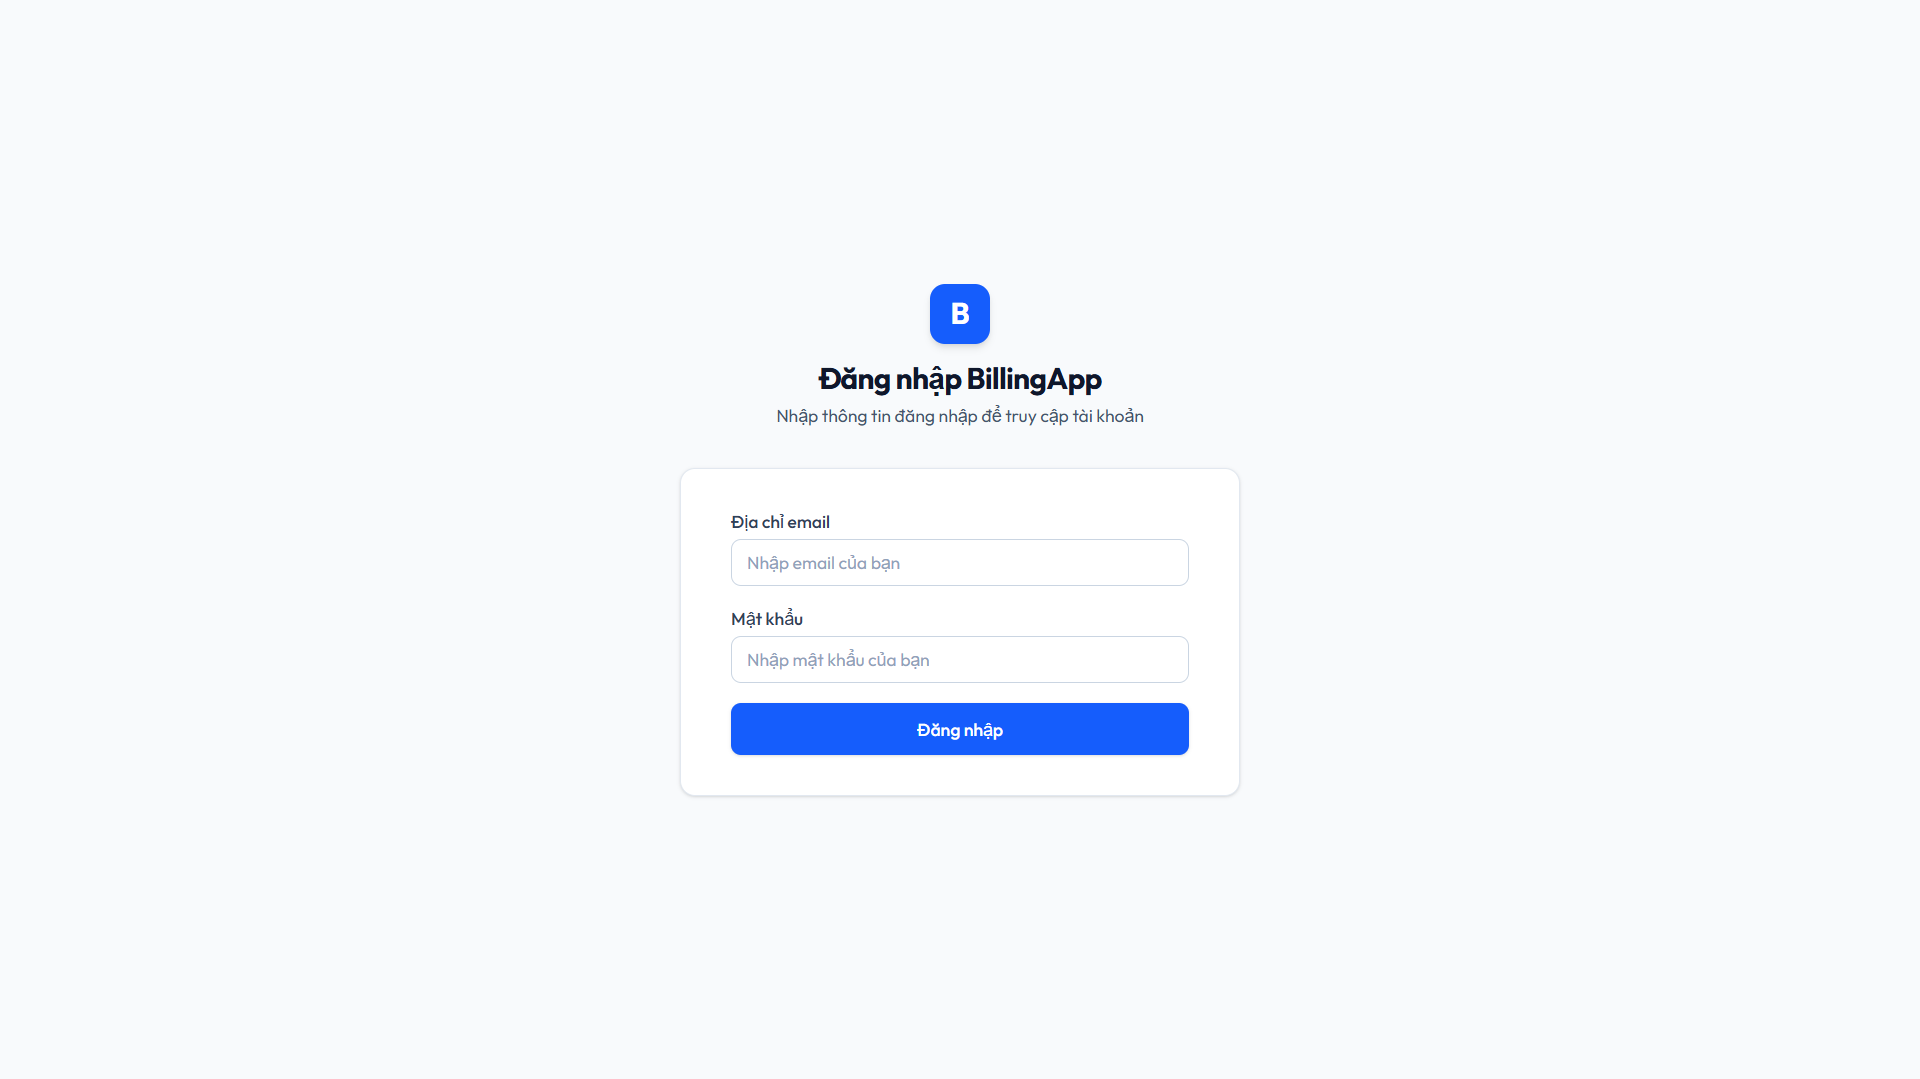
\includegraphics[width=0.75\textwidth]{images/ui_login.png}
}{
    \fbox{\parbox{0.9\textwidth}{\centering \vspace{15mm}
    \textbf{[HÌNH 3.1: GIAO DIỆN ĐĂNG NHẬP HỆ THỐNG (LOGIN VIEW)]}\\
    \textit{(Vị trí ảnh chụp: report/images/ui\_login.png)}\\
    \vspace{15mm}}}
}
\caption{Giao diện Đăng nhập và Xác thực người dùng (Auth Login)}
\label{fig:ui_login}
\end{figure}

\subsection{Màn hình Bán hàng nhanh (POS Checkout View)}
Màn hình Bán hàng nhanh (đường dẫn \texttt{/explore}) là giao diện làm việc chính của nhân viên thu ngân trong suốt ca bán (Hình \ref{fig:ui_pos_explore}):
\begin{itemize}[leftmargin=1.5cm]
    \item \textbf{Thanh phân loại danh mục (\texttt{DisplayCategories}):} Hiển thị danh sách các nhóm hàng dạng thẻ màu trực quan (như Cà phê, Trà sữa, Bánh ngọt), cho phép lọc nhanh sản phẩm theo nhóm chỉ với một cú nhấp.
    \item \textbf{Lưới hiển thị sản phẩm (\texttt{DisplayItems}):} Danh sách mặt hàng được bố trí dạng thẻ (Card) gồm hình ảnh đại diện từ AWS S3, tên mặt hàng, khoảng giá bán và số dư tồn kho khả dụng tức thời.
    \item \textbf{Thanh tìm kiếm thông minh (\texttt{SearchBox}):} Tích hợp hook tùy biến \texttt{useDebounce} (độ trễ $300$ms), hỗ trợ tìm kiếm sản phẩm theo tên hoặc quét trực tiếp mã vạch SKU bằng máy quét cầm tay.
\end{itemize}

\begin{figure}[H]
\centering
\IfFileExists{images/ui_pos_explore.png}{
    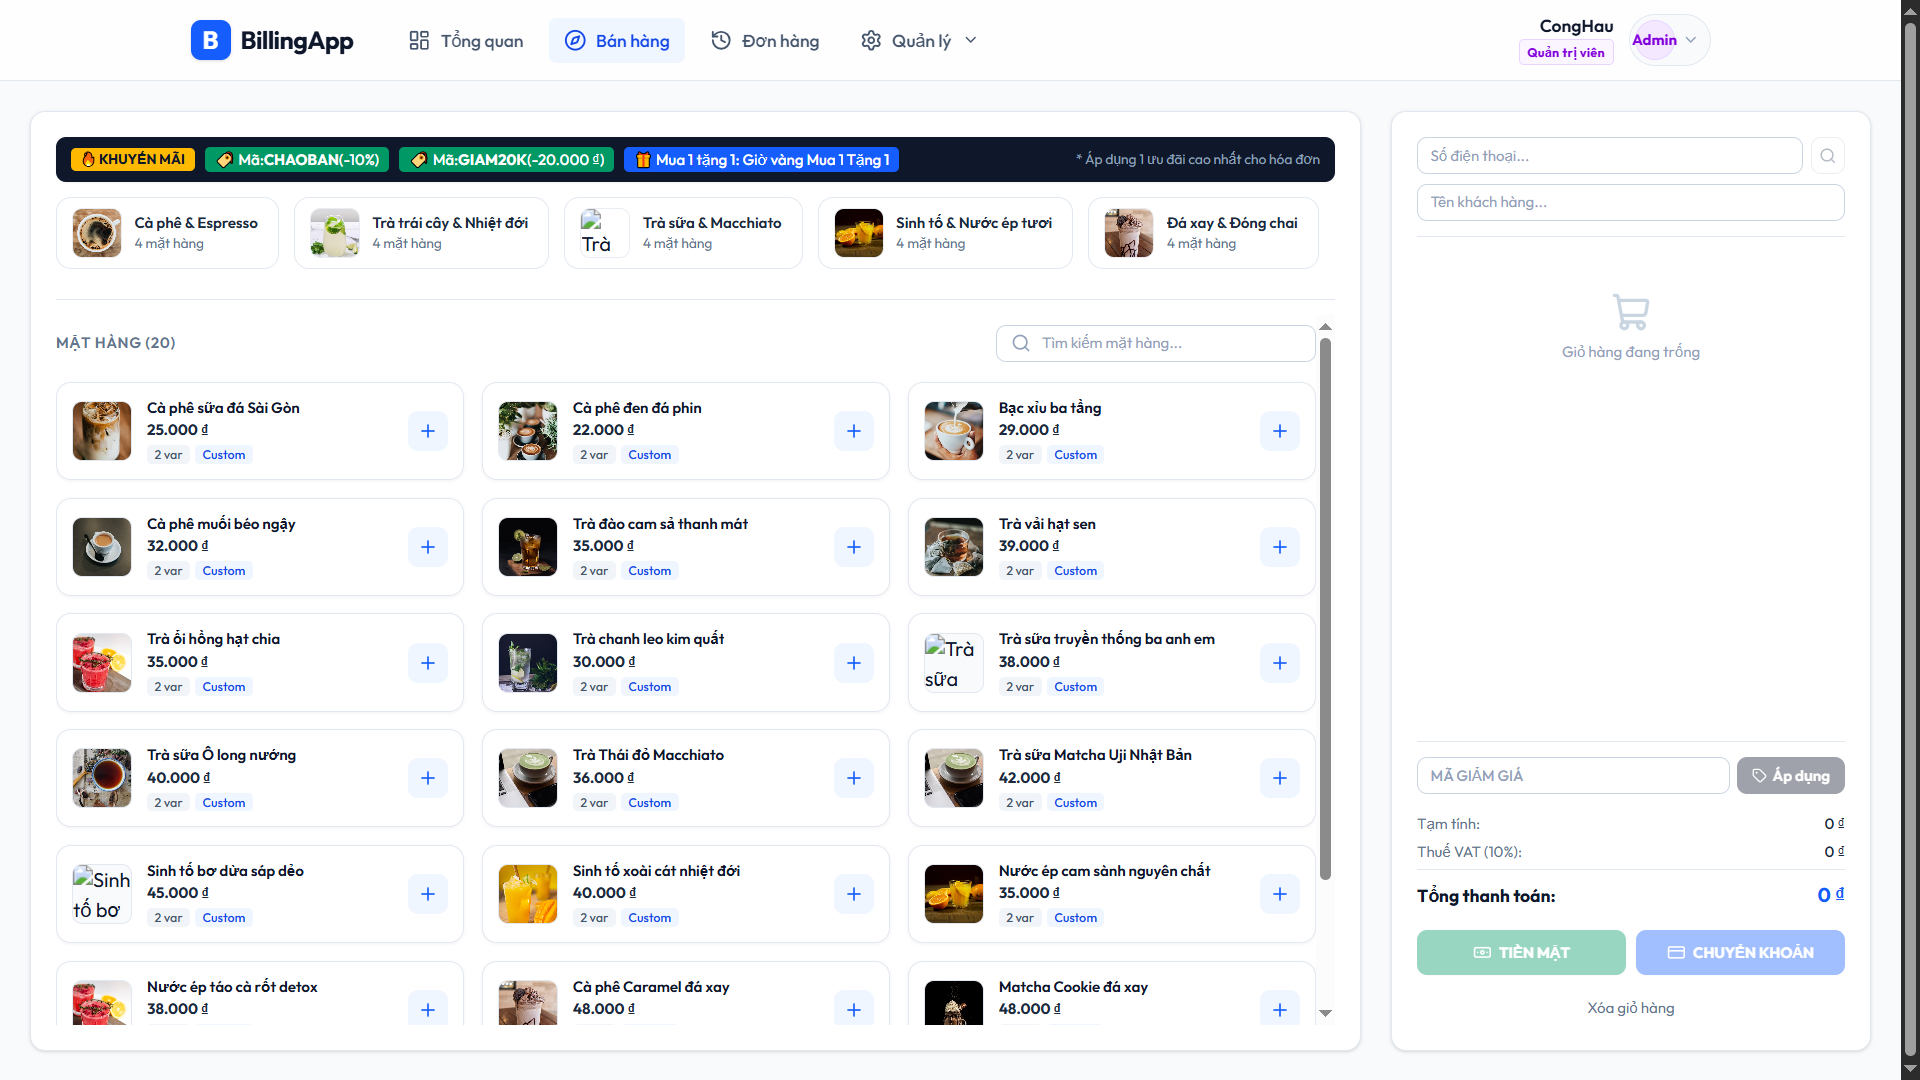
\includegraphics[width=0.92\textwidth]{images/ui_pos_explore.png}
}{
    \fbox{\parbox{0.9\textwidth}{\centering \vspace{15mm}
    \textbf{[HÌNH 3.2: GIAO DIỆN MÀN HÌNH BÁN HÀNG NHANH POS (EXPLORE VIEW)]}\\
    \textit{(Vị trí ảnh chụp: report/images/ui\_pos\_explore.png)}\\
    \vspace{15mm}}}
}
\caption{Giao diện Màn hình Bán hàng nhanh tại quầy POS}
\label{fig:ui_pos_explore}
\end{figure}

\subsection{Popup tùy biến Biến thể (Variants) và Nhóm tùy chọn (Modifiers)}
Khi thu ngân nhấp chọn một mặt hàng có cấu hình phân loại phức tạp, hệ thống mở cửa sổ con \texttt{POSItemModal} (Hình \ref{fig:ui_pos_modal}):
\begin{itemize}[leftmargin=1.5cm]
    \item \textbf{Lựa chọn biến thể SKU:} Thu ngân chọn kích thước (Size M/L) hoặc thuộc tính màu sắc. Hệ thống tự động cập nhật đơn giá cơ sở tương ứng và hiển thị số lượng hàng còn trong kho của biến thể đó.
    \item \textbf{Lựa chọn nhóm tùy chọn bổ sung (Modifiers):} Hiển thị các nhóm như Topping thêm, Mức đá, Mức đường. Hệ thống tự động kiểm tra các ràng buộc: số lượng chọn tối thiểu (\texttt{minSelections}) và tối đa (\texttt{maxSelections}). Khi chọn thêm Topping (ví dụ: Trân châu trắng +$10.000$đ), tổng giá tiền trên modal tự động cộng dồn theo thời gian thực.
    \item Nhấn nút ''Thêm vào giỏ hàng'', sản phẩm được đưa vào giỏ với mã định danh kết hợp duy nhất: \texttt{\$\{itemId\}\_\$\{variantId\}\_\$\{modifierIds\}}.
\end{itemize}

\begin{figure}[H]
\centering
\IfFileExists{images/ui_pos_modal.png}{
    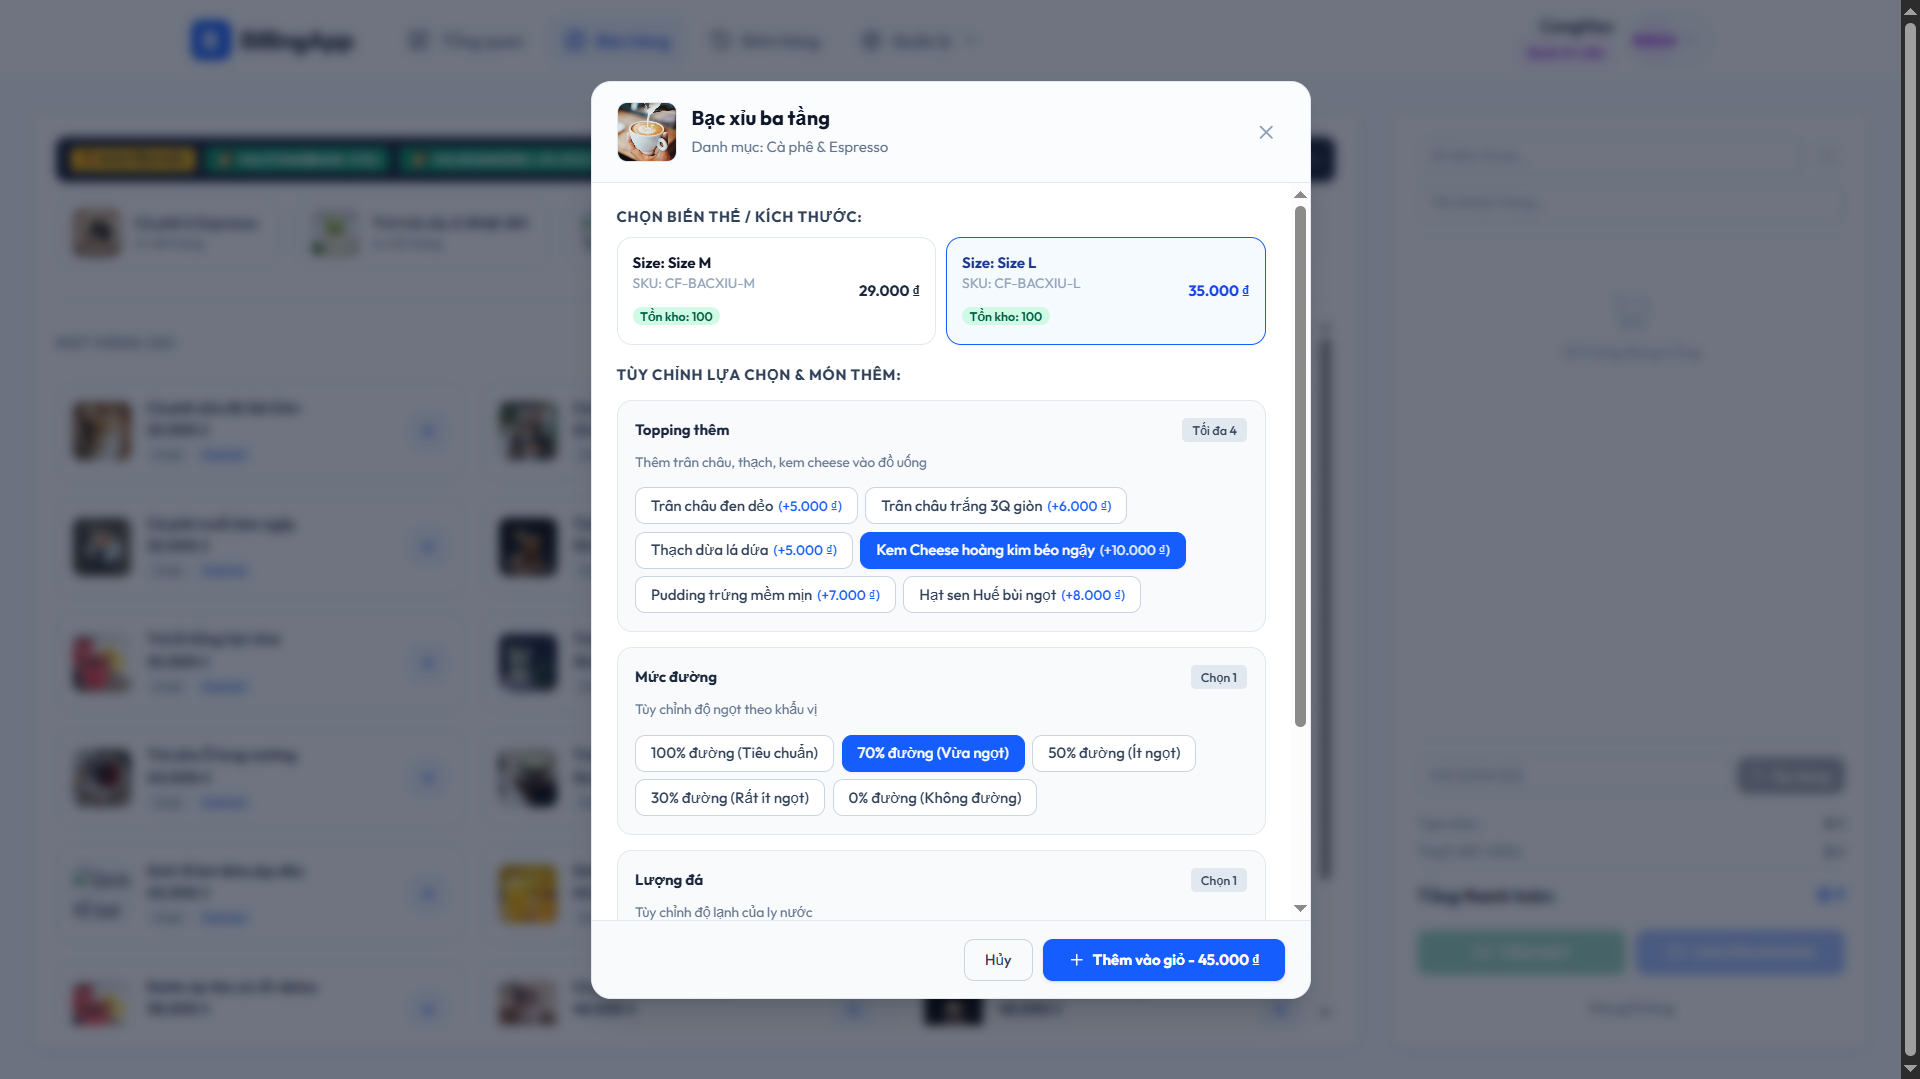
\includegraphics[width=0.88\textwidth]{images/ui_pos_modal.png}
}{
    \fbox{\parbox{0.9\textwidth}{\centering \vspace{12mm}
    \textbf{[HÌNH 3.3: POPUP TÙY CHỌN BIẾN THỂ SKU VÀ NHÓM TOPPING MODIFIERS]}\\
    \textit{(Vị trí ảnh chụp: report/images/ui\_pos\_modal.png)}\\
    \vspace{12mm}}}
}
\caption{Giao diện Popup tùy chọn biến thể SKU và Modifiers}
\label{fig:ui_pos_modal}
\end{figure}

\subsection{Quản lý Giỏ hàng và Nhận diện Khách hàng thân thiết CRM}
Bên phải màn hình bán hàng là bảng tóm tắt đơn hàng (\texttt{CartSummary}):
\begin{itemize}[leftmargin=1.5cm]
    \item Danh sách các dòng hàng đã chọn kèm số lượng, nút tăng/giảm nhanh (+/-) và nút xóa dòng hàng.
    \item \textbf{Biểu mẫu khách hàng thân thiết (\texttt{CustomerForm}):} Thu ngân nhập số điện thoại khách hàng. Hook gọi API \texttt{GET /customers/by-phone/\{phone\}}. Nếu khách hàng đã tồn tại, hệ thống hiển thị ngay tên khách hàng, tổng tiền tích lũy và số điểm thưởng. Nếu là khách hàng mới, hệ thống cho phép tạo nhanh tài khoản CRM ngay tại quầy mà không làm gián đoạn giỏ hàng.
    \item \textbf{Tự động đánh giá khuyến mãi:} Hệ thống liên tục gửi dữ liệu giỏ hàng tới endpoint \texttt{/promotions/evaluate} để áp dụng mức giảm giá cao nhất (Happy Hour hoặc Coupon) và hiển thị rõ ràng số tiền được giảm trừ.
\end{itemize}

\subsection{Thanh toán kép: Tiền mặt và VietQR PayOS thời gian thực}
Thu ngân có thể lựa chọn 1 trong 2 phương thức thanh toán linh hoạt:
\begin{enumerate}[label=\arabic*., leftmargin=1.5cm]
    \item \textbf{Thanh toán Tiền mặt (CASH):} Thu ngân nhập số tiền khách đưa (có các nút gợi ý tiền mặt nhanh: 50k, 100k, 200k, 500k). Hệ thống tự động tính toán số tiền thừa phải trả lại khách và mở ngay cửa sổ in hóa đơn bán lẻ.
    \item \textbf{Thanh toán chuyển khoản VietQR PayOS (PAYOS):}
    \begin{itemize}
        \item Hệ thống kích hoạt cửa sổ \texttt{PaymentQRCode} (Hình \ref{fig:ui_payment_qr}), hiển thị mã VietQR động theo chuẩn NAPAS có nhúng chính xác số tiền cần trả và mã đơn hàng đã được khóa bảo vệ.
        \item Front-end kích hoạt hook \texttt{usePolledOrderData} thăm dò tự động mỗi 3 giây. Ngay khi khách hàng chuyển khoản thành công và PayOS gửi Webhook, màn hình tự động chuyển sang trạng thái \texttt{COMPLETED}.
        \item \textbf{Quy trình chuyển sang tiền mặt (\textit{Switch to Cash}):} Nếu khách hàng gặp sự cố mạng di động, thu ngân có thể nhấn nút \textit{''Chuyển sang tiền mặt''}. Hệ thống gọi API hủy link PayOS và ghi nhận thanh toán tiền mặt tức thì.
    \end{itemize}
\end{enumerate}

\begin{figure}[H]
\centering
\IfFileExists{images/ui_payment_qr.png}{
    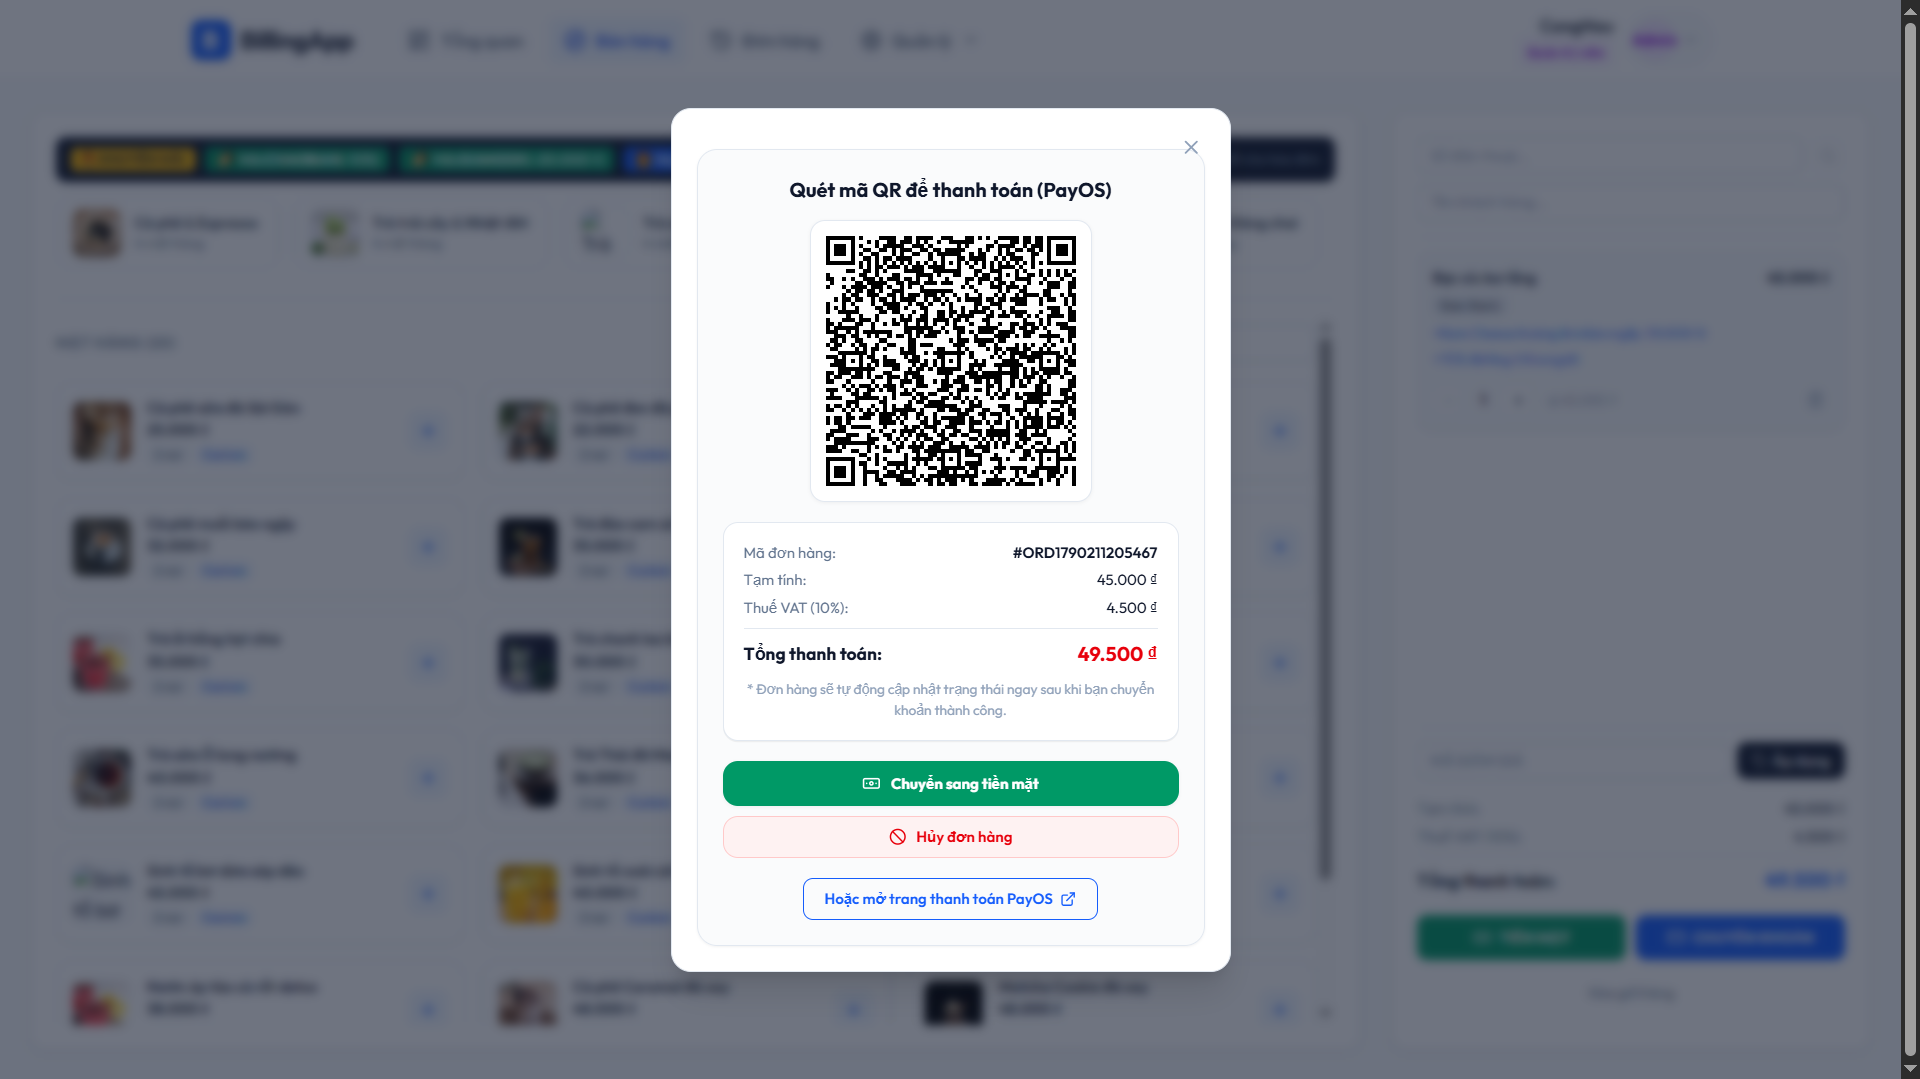
\includegraphics[width=0.88\textwidth]{images/ui_payment_qr.png}
}{
    \fbox{\parbox{0.9\textwidth}{\centering \vspace{15mm}
    \textbf{[HÌNH 3.4: CỬA SỔ QUÉT MÃ THANH TOÁN VIETQR PAYOS THỜI GIAN THỰC]}\\
    \textit{(Vị trí ảnh chụp: report/images/ui\_payment\_qr.png)}\\
    \vspace{15mm}}}
}
\caption{Giao diện Quét mã thanh toán VietQR động tích hợp PayOS}
\label{fig:ui_payment_qr}
\end{figure}

\subsection{Mẫu in hóa đơn bán lẻ nhiệt 80mm}
Cửa sổ \texttt{ReceiptPopup} (Hình \ref{fig:ui_receipt}) được thiết kế chuẩn mực theo tiêu chuẩn giấy in nhiệt 80mm thông dụng tại các siêu thị và nhà hàng:
\begin{itemize}[leftmargin=1.5cm]
    \item Phần đầu: Tên cửa hàng, địa chỉ, số điện thoại hotline và số hiệu hóa đơn (\texttt{order\_code}).
    \item Phần thân: Bảng danh sách các mặt hàng, biến thể SKU, danh sách Modifier đính kèm, số lượng, đơn giá và thành tiền.
    \item Phần chân: Tổng tiền hàng (\texttt{subtotal}), tiền chiết khấu khuyến mãi (\texttt{discountAmount}), tiền thuế VAT 10\% (\texttt{tax}), tổng thanh toán cuối cùng (\texttt{grandTotal}), phương thức thanh toán, tiền khách đưa và tiền thừa thối lại.
    \item Tích hợp lệnh gọi in trực tiếp trình duyệt (\texttt{window.print()}) với định dạng \texttt{@media print} tối ưu độ sắc nét cho đầu in nhiệt.
\end{itemize}

\begin{figure}[H]
\centering
\IfFileExists{images/ui_receipt.png}{
    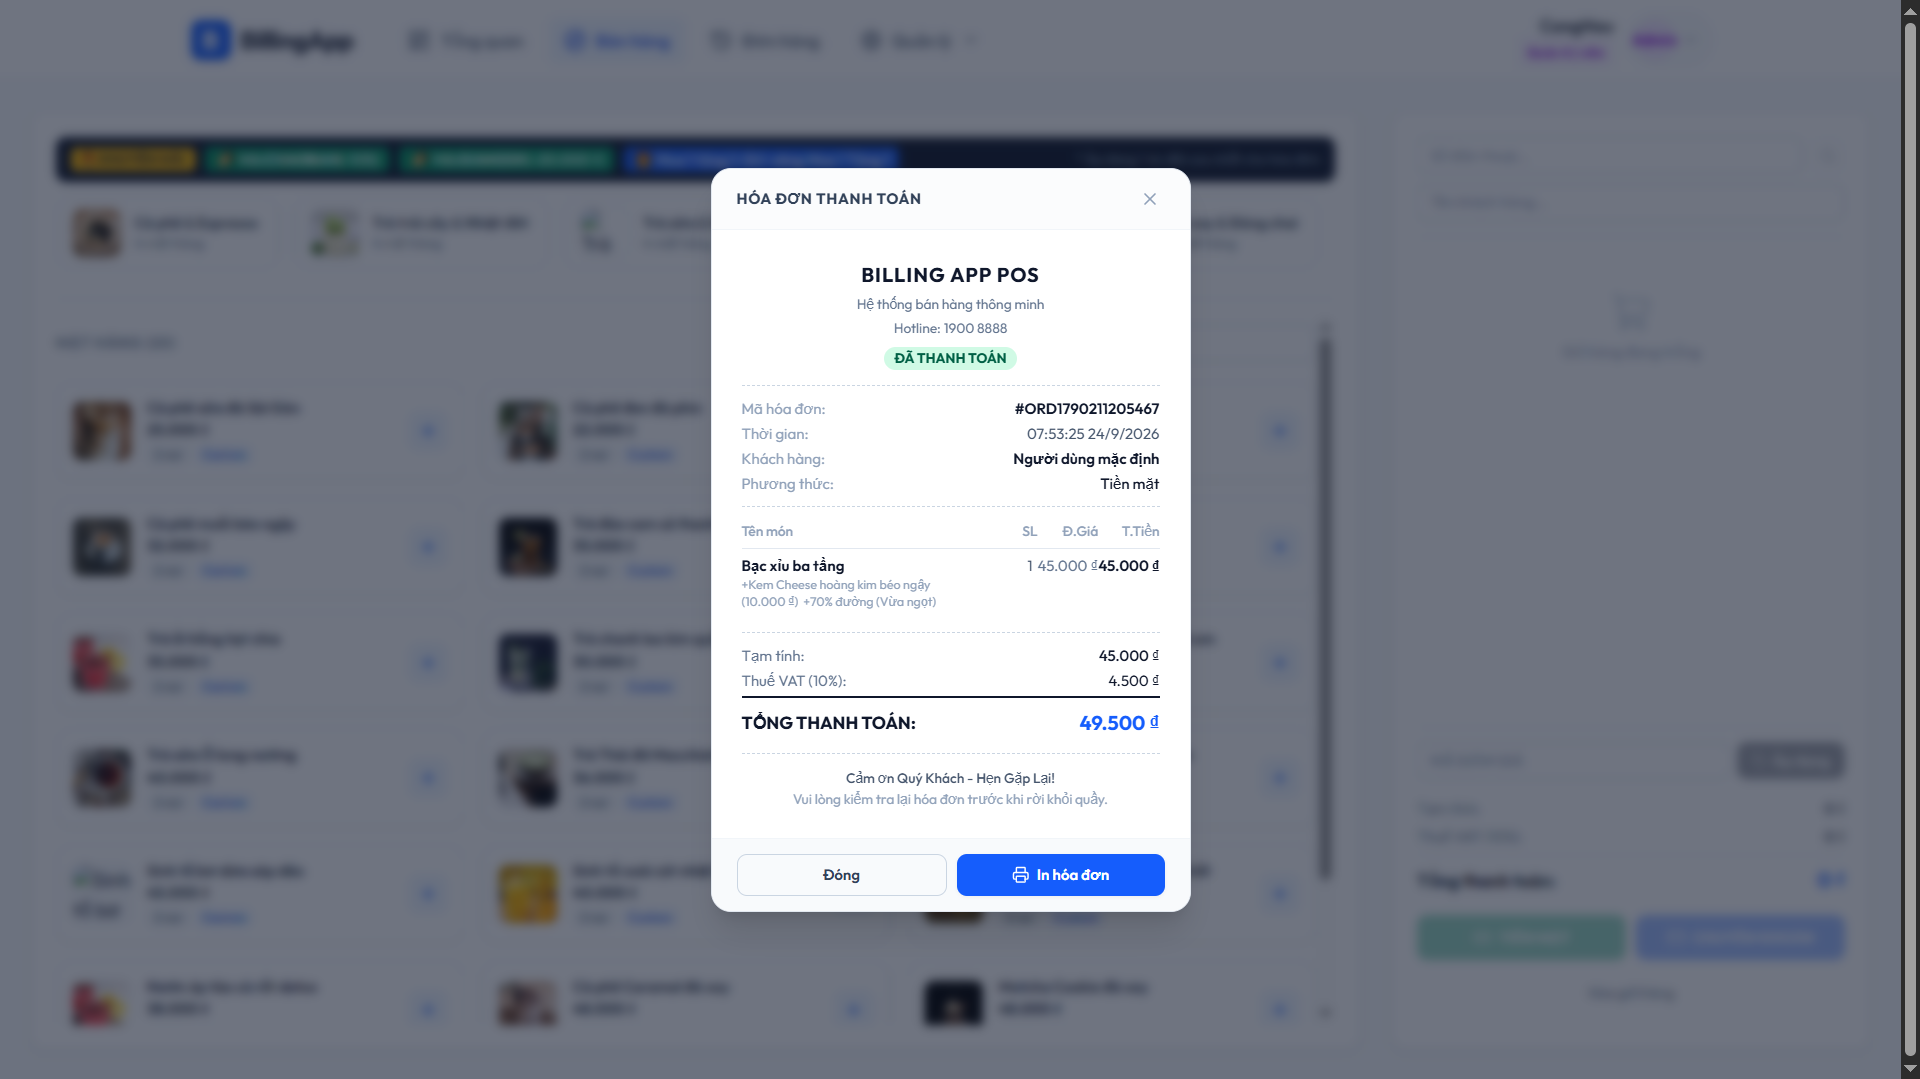
\includegraphics[width=0.85\textwidth]{images/ui_receipt.png}
}{
    \fbox{\parbox{0.9\textwidth}{\centering \vspace{15mm}
    \textbf{[HÌNH 3.5: MẪU HÓA ĐƠN BÁN LẺ IN NHIỆT 80MM (THERMAL RECEIPT)]}\\
    \textit{(Vị trí ảnh chụp: report/images/ui\_receipt.png)}\\
    \vspace{15mm}}}
}
\caption{Mẫu Hóa đơn bán lẻ in nhiệt 80mm chuẩn hóa}
\label{fig:ui_receipt}
\end{figure}

\subsection{Màn hình Lịch sử đơn hàng và Hủy đơn bù trừ kho}
Màn hình Lịch sử đơn hàng (\texttt{OrderHistory} - Hình \ref{fig:ui_order_history}) cung cấp các công cụ quản lý sau bán hàng:
\begin{itemize}[leftmargin=1.5cm]
    \item Danh sách phân trang toàn bộ các hóa đơn đã phát sinh, hỗ trợ bộ lọc theo trạng thái: \texttt{PENDING}, \texttt{COMPLETED}, \texttt{CANCELLED}.
    \item Xem lại chi tiết đơn hàng và in lại hóa đơn (Re-print receipt) bất kỳ lúc nào.
    \item \textbf{Cơ chế bảo vệ kế toán nghiêm ngặt:} Đơn hàng đã \texttt{COMPLETED} không có nút xóa nhằm chống gian lận doanh số. Nút ''Hủy đơn'' chỉ xuất hiện đối với đơn hàng đang \texttt{PENDING}. Khi xác nhận hủy, hệ thống kích hoạt giao dịch bù trừ kho (Stock In) và hoàn lại số lượt dùng voucher khuyến mãi.
\end{itemize}

\begin{figure}[H]
\centering
\IfFileExists{images/ui_order_history.png}{
    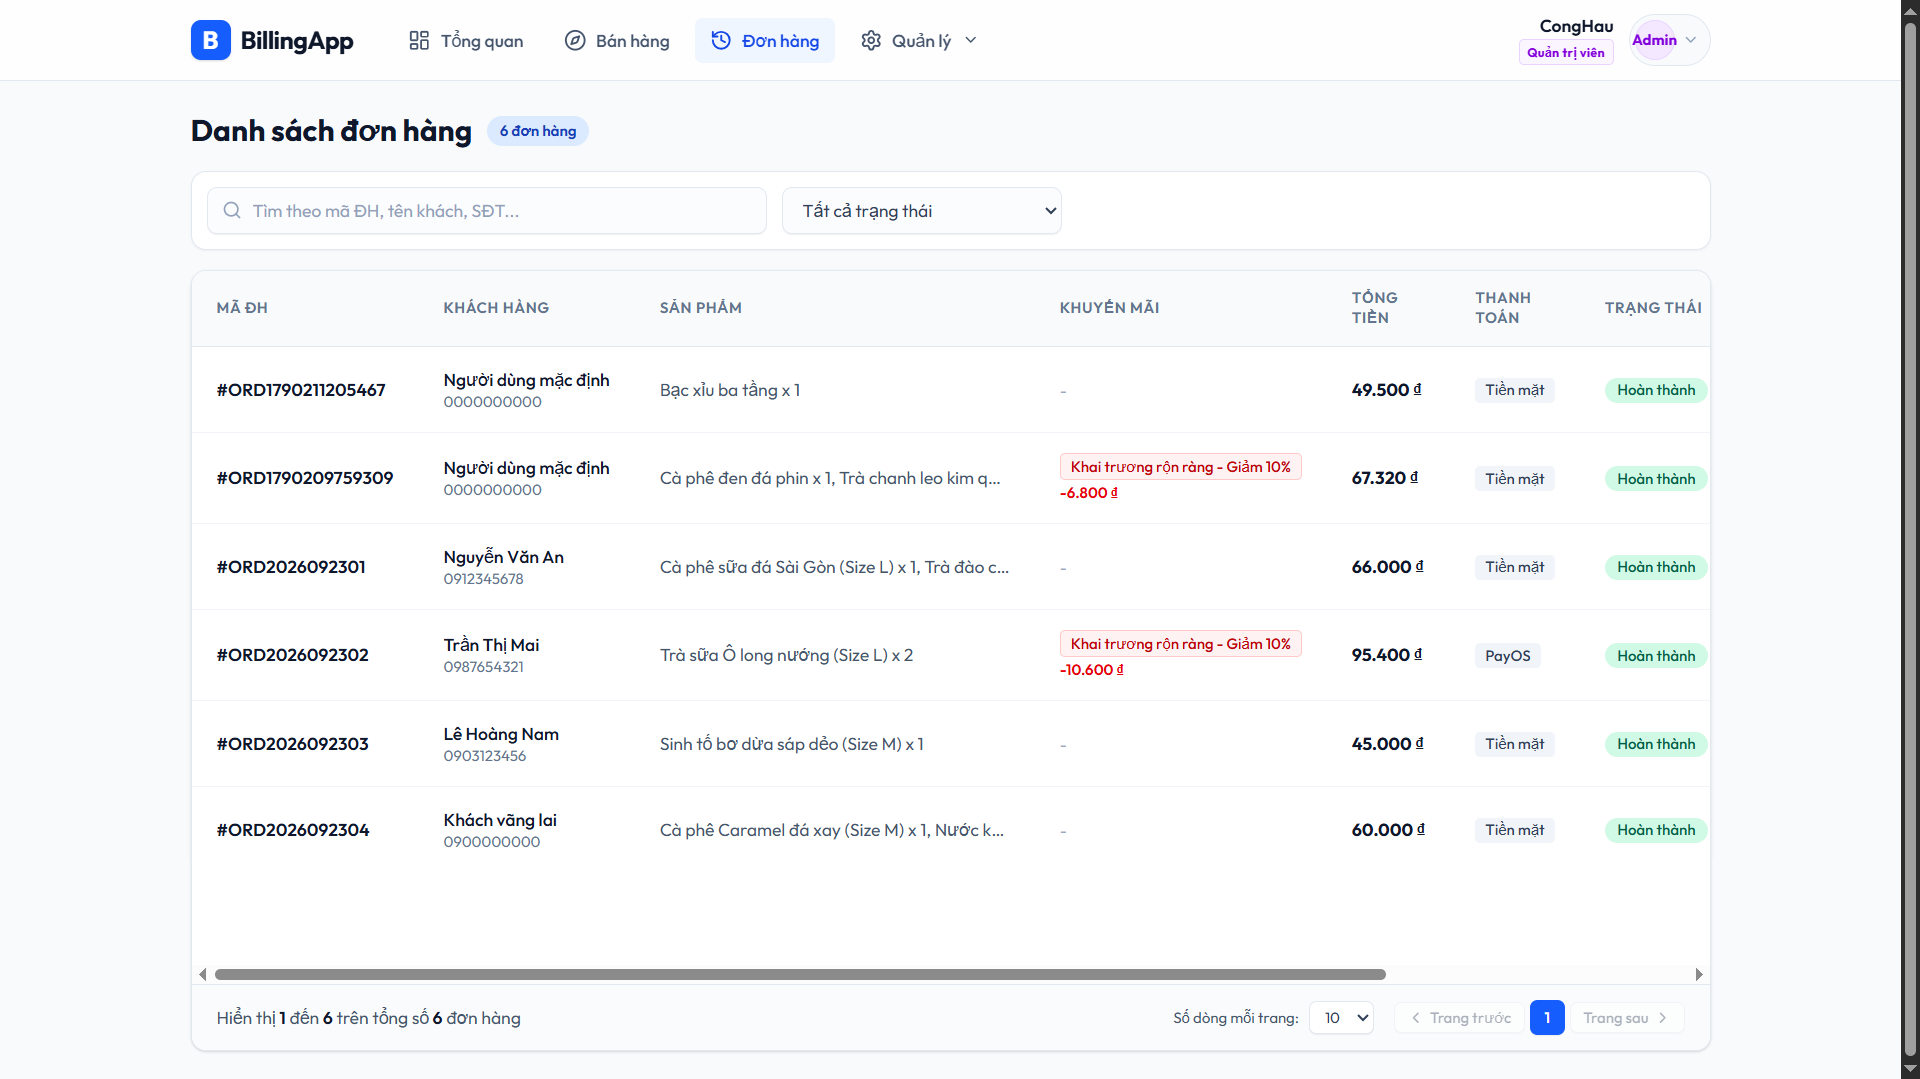
\includegraphics[width=0.92\textwidth]{images/ui_order_history.png}
}{
    \fbox{\parbox{0.9\textwidth}{\centering \vspace{15mm}
    \textbf{[HÌNH 3.6: GIAO DIỆN LỊCH SỬ ĐƠN HÀNG VÀ THEO DÕI TRẠNG THÁI]}\\
    \textit{(Vị trí ảnh chụp: report/images/ui\_order\_history.png)}\\
    \vspace{15mm}}}
}
\caption{Giao diện Quản lý Lịch sử đơn hàng và Trạng thái thanh toán}
\label{fig:ui_order_history}
\end{figure}

% ==============================================================================
\section{Hiện thực phân hệ Quản trị (Dành cho Admin/Quản lý)}
\label{sec:hien_thuc_quan_tri}

Phân hệ Quản trị được bảo vệ bởi bộ định tuyến an ninh \texttt{AdminRoute}, chỉ cho phép tài khoản có vai trò \texttt{ROLE\_ADMIN} truy cập.

\subsection{Bảng điều khiển chỉ số kinh doanh và Báo cáo Doanh thu (Dashboard KPI)}
Trang chủ Quản trị (\texttt{/dashboard} - Hình \ref{fig:ui_dashboard}) cung cấp bức tranh toàn cảnh về hiệu quả kinh doanh của cửa hàng trong ngày và hỗ trợ báo cáo thống kê doanh thu chuyên sâu:
\begin{itemize}[leftmargin=1.5cm]
    \item \textbf{Thẻ đo lường KPI doanh thu:} Tổng doanh thu ngày/tuần/tháng hiện tại, tỉ lệ tăng trưởng so với kỳ trước cùng khoảng thời gian, biểu thị bằng mũi tên xu hướng tăng/giảm kèm phần trăm.
    \item \textbf{Thẻ đếm số lượng hóa đơn:} Tổng số đơn hàng hoàn tất (\texttt{COMPLETED}), số đơn đang chờ (\texttt{PENDING}) và số đơn đã hủy (\texttt{CANCELLED}) trong khoảng thời gian.
    \item \textbf{Bảng danh sách đơn hàng mới nhất:} Hiển thị các giao dịch vừa phát sinh theo thời gian thực kèm mã hóa đơn và trạng thái thanh toán.
    \item \textbf{Bảng xếp hạng sản phẩm bán chạy (Top Items):} Danh sách các sản phẩm có số lượng bán cao nhất, tổng hợp từ bảng \texttt{tbl\_order\_items} theo biến thể SKU.
    \item \textbf{Cảnh báo tồn kho thấp (Low Stock Alert):} Liệt kê các biến thể có số dư \texttt{cachedStockQuantity} dưới ngưỡng cảnh báo, giúp quản lý chủ động lên kế hoạch nhập hàng kịp thời.
\end{itemize}

\begin{figure}[H]
\centering
\IfFileExists{images/ui_dashboard.png}{
    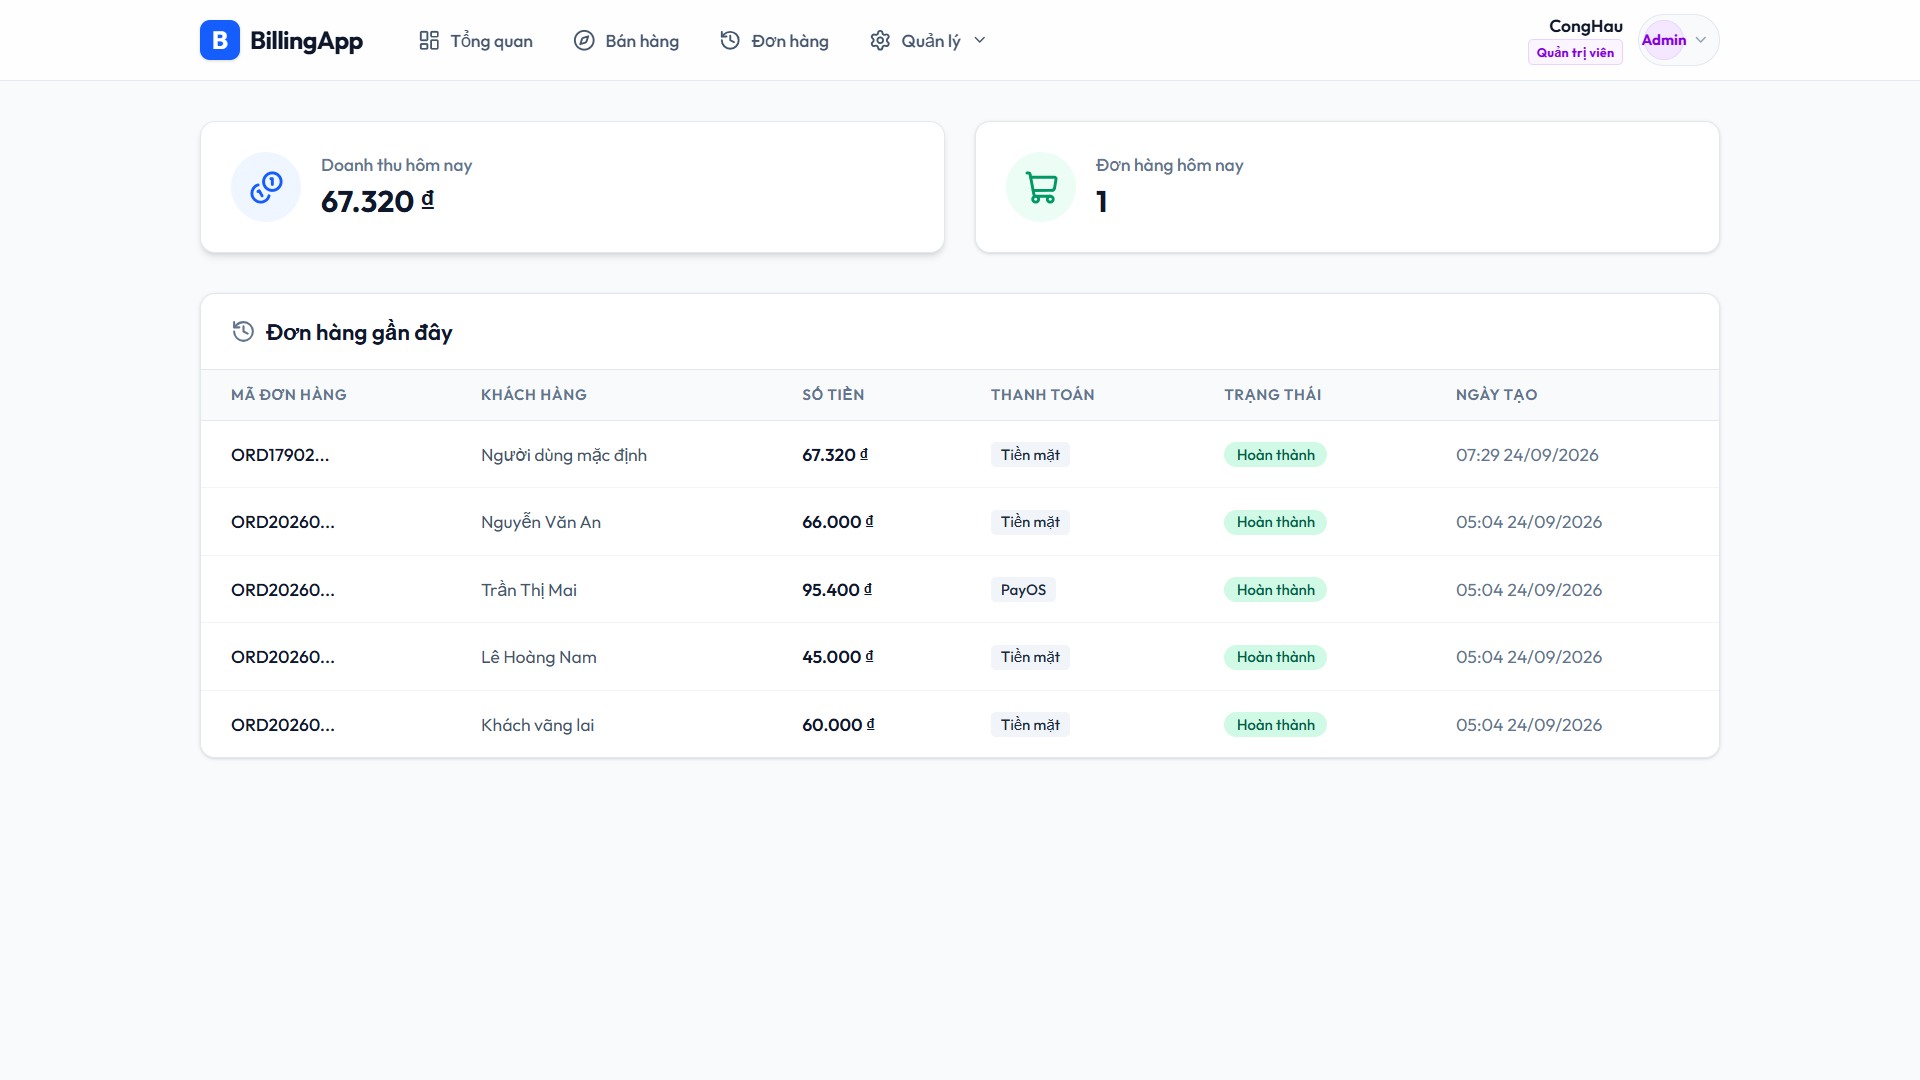
\includegraphics[width=0.92\textwidth]{images/ui_dashboard.png}
}{
    \fbox{\parbox{0.9\textwidth}{\centering \vspace{15mm}
    \textbf{[HÌNH 3.7: BẢNG ĐIỀU KHIỂN CHỈ SỐ KINH DOANH VÀ BÁO CÁO DOANH THU (DASHBOARD)]}\\
    \textit{(Vị trí ảnh chụp: report/images/ui\_dashboard.png)}\\
    \vspace{15mm}}}
}
\caption{Giao diện Bảng điều khiển kinh doanh tổng quan và Báo cáo Doanh thu (Dashboard)}
\label{fig:ui_dashboard}
\end{figure}

\subsection{Quản trị Danh mục hàng hóa (Categories)}
Giao diện Quản trị Danh mục (\texttt{/categories} - Hình \ref{fig:ui_manage_categories}) cho phép người quản lý tổ chức cây danh mục mặt hàng theo từng nhóm nghiệp vụ:
\begin{itemize}[leftmargin=1.5cm]
    \item Danh sách phân loại các nhóm sản phẩm (Cà phê, Trà hoa quả, Đồ ăn nhanh, Bánh ngọt).
    \item Thêm mới, cập nhật tên danh mục, biểu tượng nhận diện và trạng thái kích hoạt hiển thị tại quầy POS.
    \item Ràng buộc toàn vẹn: Không cho phép xóa danh mục khi đang có sản phẩm con liên kết (\texttt{ON DELETE RESTRICT}).
\end{itemize}

\begin{figure}[H]
\centering
\IfFileExists{images/ui_manage_categories.png}{
    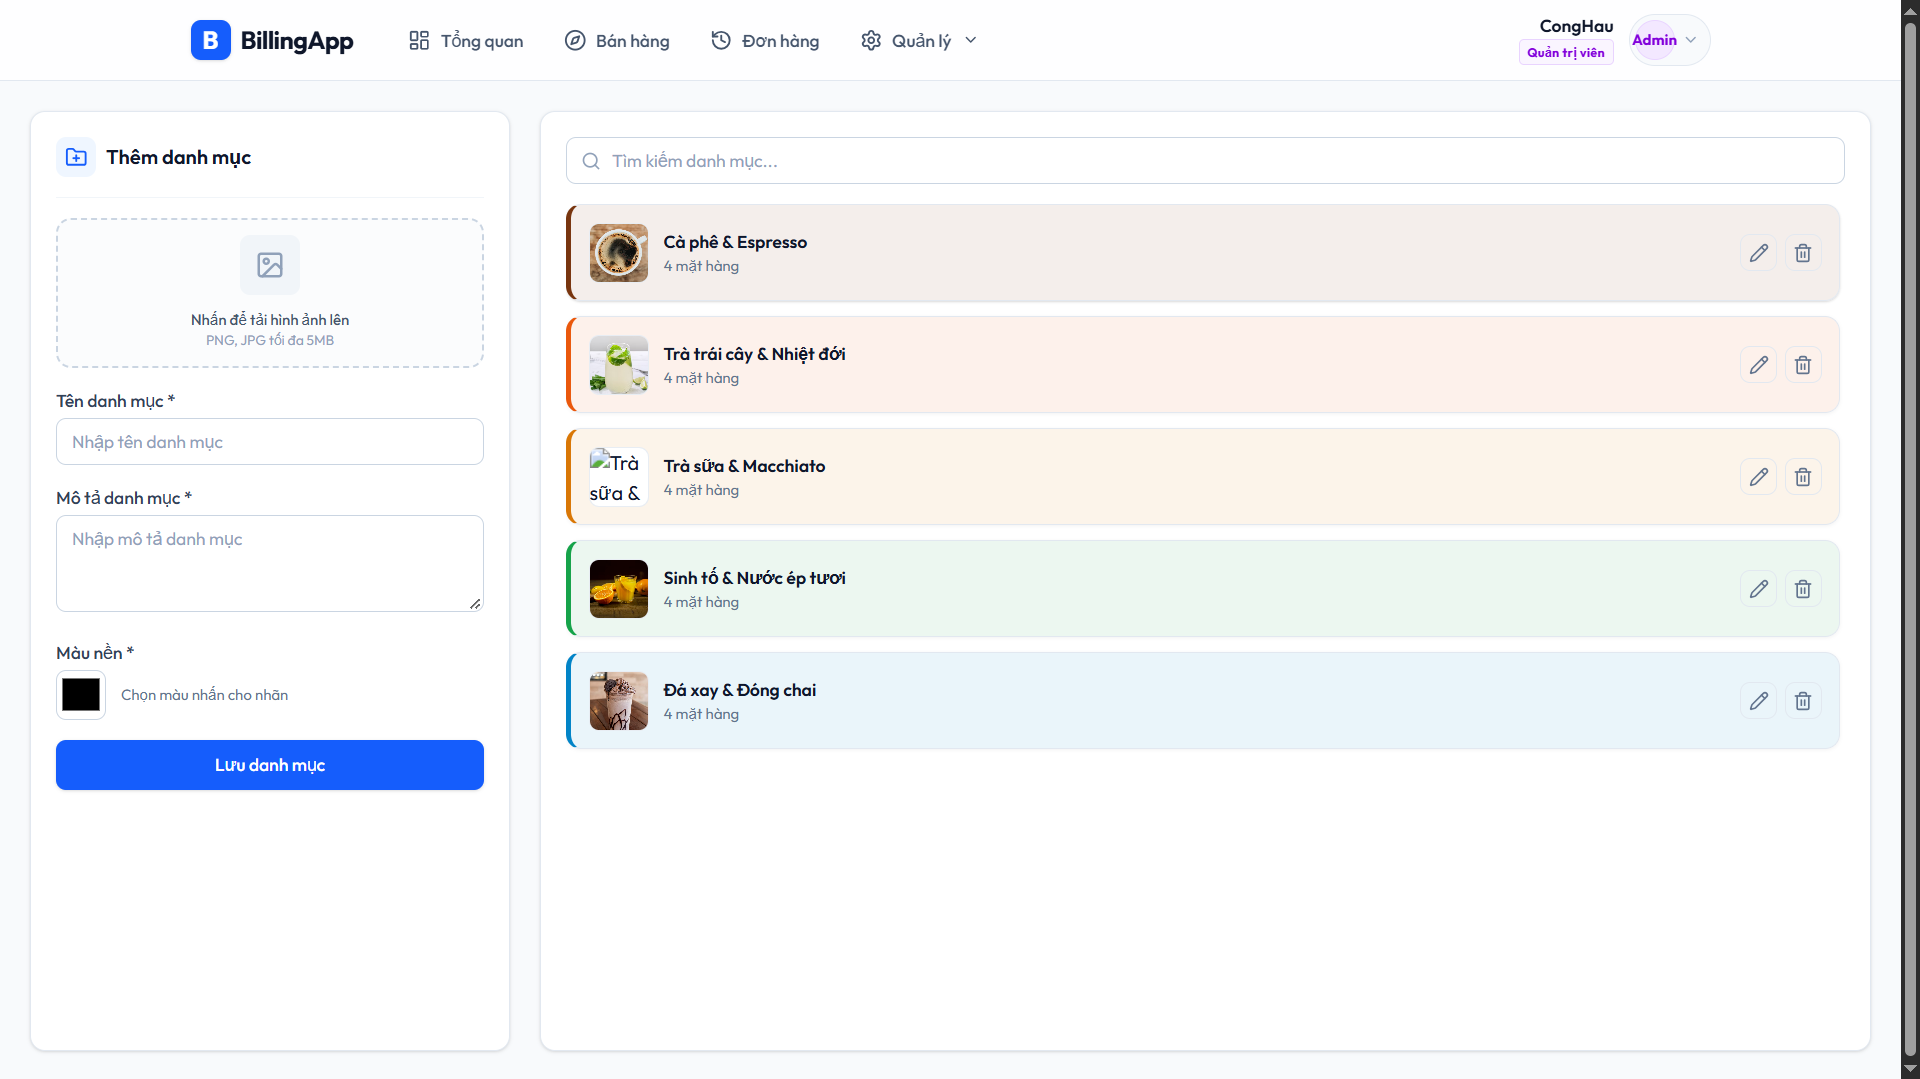
\includegraphics[width=0.92\textwidth]{images/ui_manage_categories.png}
}{
    \fbox{\parbox{0.9\textwidth}{\centering \vspace{15mm}
    \textbf{[HÌNH 3.8: GIAO DIỆN QUẢN TRỊ DANH MỤC HÀNG HÓA]}\\
    \textit{(Vị trí ảnh chụp: report/images/ui\_manage\_categories.png)}\\
    \vspace{15mm}}}
}
\caption{Giao diện Quản trị Danh mục hàng hóa (Categories)}
\label{fig:ui_manage_categories}
\end{figure}

\subsection{Quản lý Sản phẩm, Biến thể SKU và Tải ảnh AWS S3}
Trang Quản lý Sản phẩm (\texttt{/items} - Hình \ref{fig:ui_manage_items}) hỗ trợ:
\begin{itemize}[leftmargin=1.5cm]
    \item Thêm mới và cập nhật sản phẩm có kèm tệp hình ảnh tải lên kho đám mây AWS S3.
    \item Tạo động danh sách các biến thể phân loại (SKU) với bảng thuộc tính động dạng JSON (như Size: L, Màu: Đỏ).
    \item Gán các nhóm tùy chọn Modifier vào từng sản phẩm tương ứng.
\end{itemize}

\begin{figure}[H]
\centering
\IfFileExists{images/ui_manage_items.png}{
    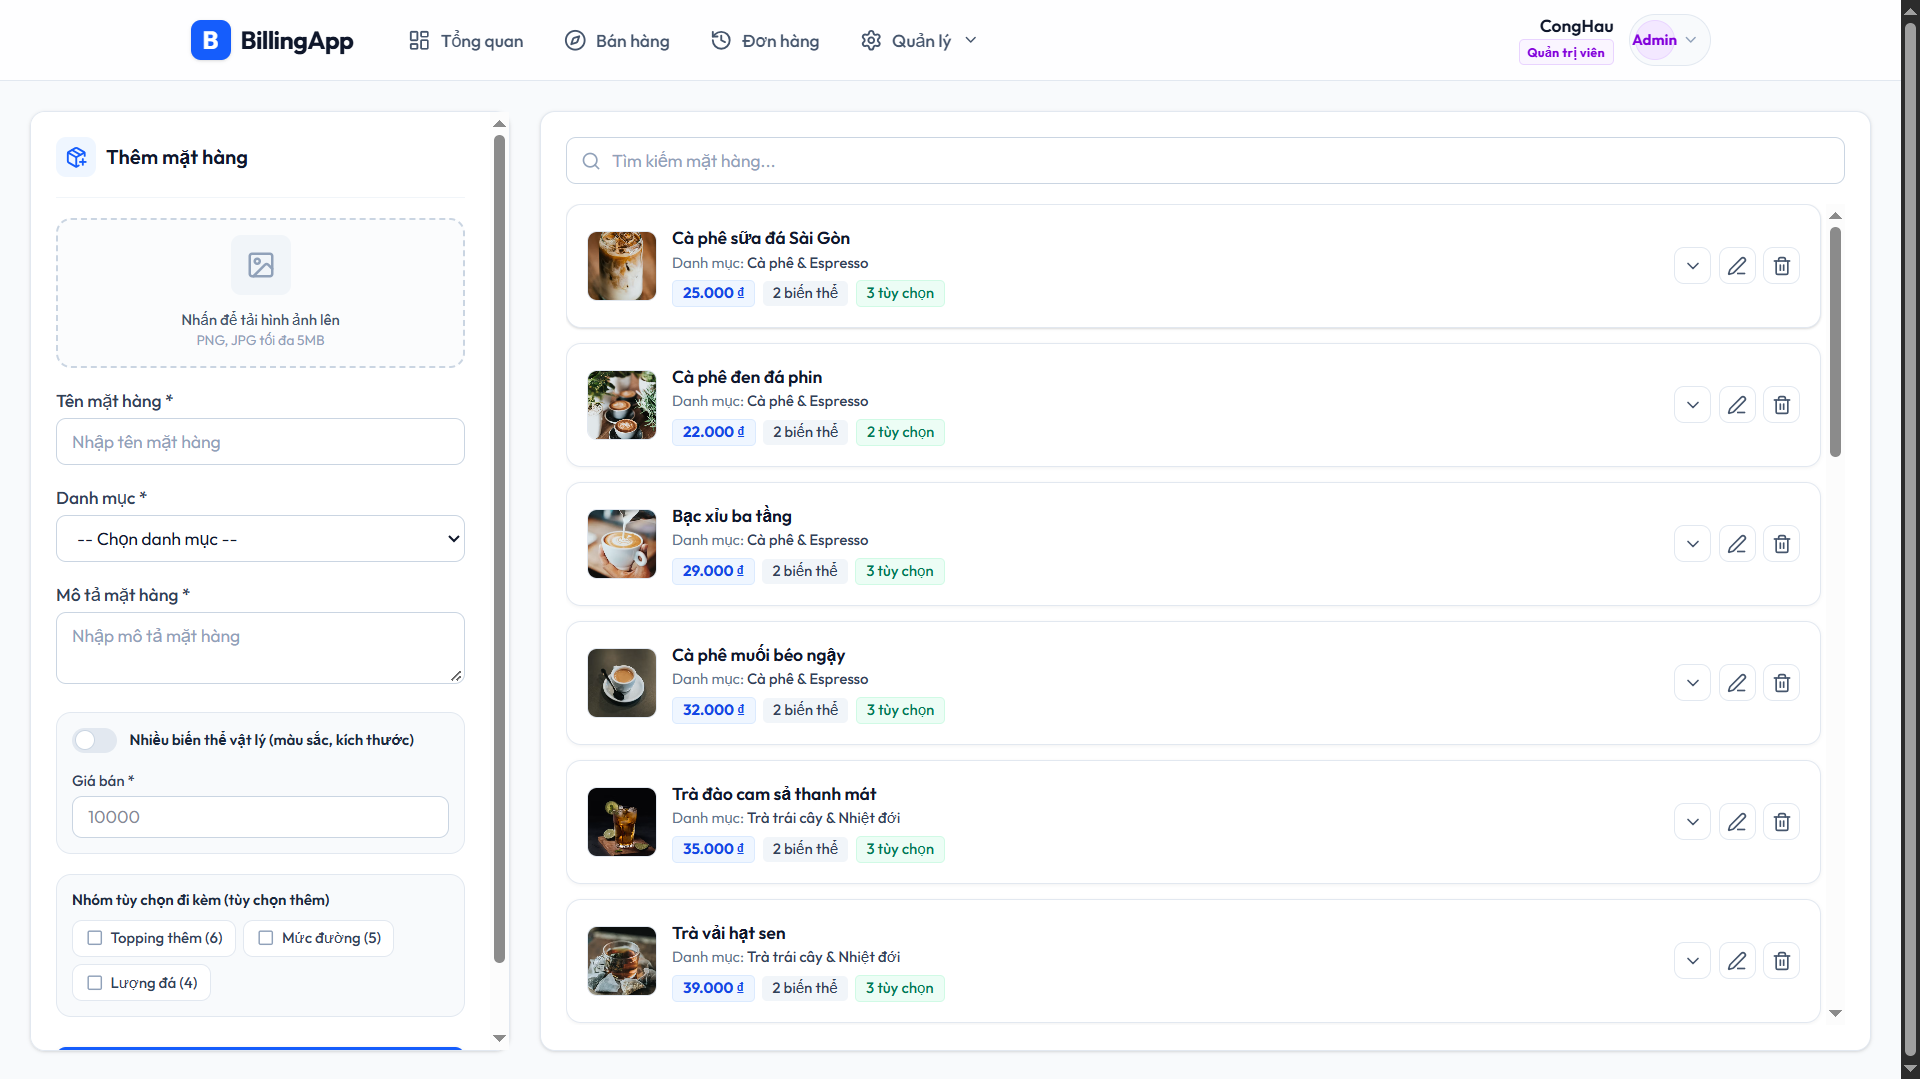
\includegraphics[width=0.92\textwidth]{images/ui_manage_items.png}
}{
    \fbox{\parbox{0.9\textwidth}{\centering \vspace{15mm}
    \textbf{[HÌNH 3.9: GIAO DIỆN QUẢN LÝ SẢN PHẨM VÀ CÁC BIẾN THỂ PHÂN LOẠI]}\\
    \textit{(Vị trí ảnh chụp: report/images/ui\_manage\_items.png)}\\
    \vspace{15mm}}}
}
\caption{Giao diện Quản lý danh mục Sản phẩm và Biến thể SKU}
\label{fig:ui_manage_items}
\end{figure}

\subsection{Quản trị Nhóm tùy chọn bổ sung (Modifiers)}
Giao diện Quản lý Nhóm tùy chọn (\texttt{/modifiers} - Hình \ref{fig:ui_manage_modifiers}) hỗ trợ định nghĩa các nhóm phụ phí và gia giảm:
\begin{itemize}[leftmargin=1.5cm]
    \item Thiết lập các nhóm như Topping thêm, Mức đá (0\%, 50\%, 100\%), Mức đường (0\%, 30\%, 70\%, 100\%).
    \item Cấu hình số lựa chọn tối thiểu (\texttt{minSelections}) và tối đa (\texttt{maxSelections}).
    \item Danh sách các tùy chọn chi tiết bên trong nhóm kèm mức điều chỉnh giá (\texttt{priceAdjustment}).
\end{itemize}

\begin{figure}[H]
\centering
\IfFileExists{images/ui_manage_modifiers.png}{
    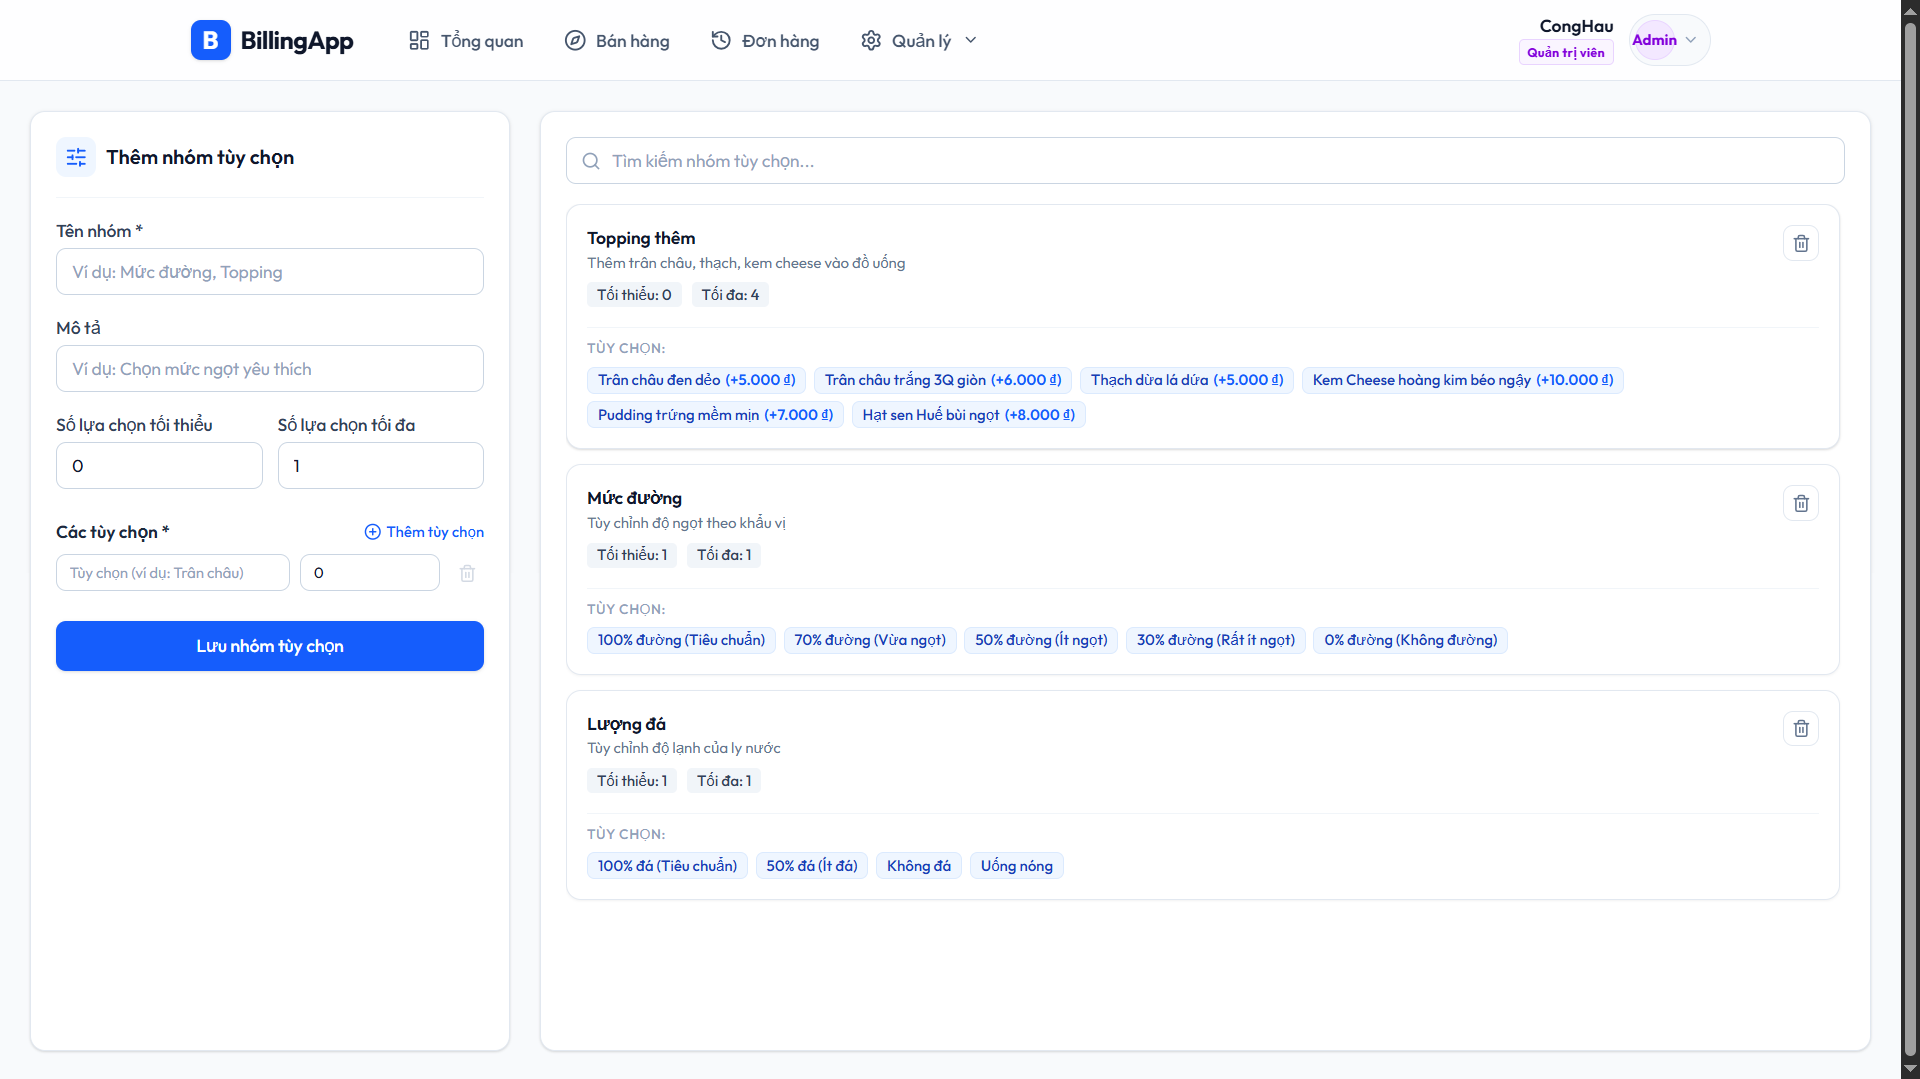
\includegraphics[width=0.92\textwidth]{images/ui_manage_modifiers.png}
}{
    \fbox{\parbox{0.9\textwidth}{\centering \vspace{15mm}
    \textbf{[HÌNH 3.10: GIAO DIỆN QUẢN TRỊ NHÓM TÙY CHỌN BỔ SUNG (MODIFIERS)]}\\
    \textit{(Vị trí ảnh chụp: report/images/ui\_manage\_modifiers.png)}\\
    \vspace{15mm}}}
}
\caption{Giao diện Quản trị Nhóm tùy chọn bổ sung (Modifiers)}
\label{fig:ui_manage_modifiers}
\end{figure}

\subsection{Quản lý Kho sổ cái và Kiểm kê cân bằng tồn kho}
Cửa sổ \texttt{StockOperationModal} (Hình \ref{fig:ui_stock_operation}) cung cấp các công cụ quản lý kho chuyên nghiệp:
\begin{itemize}[leftmargin=1.5cm]
    \item \textbf{Nhập kho (Stock IN):} Tăng số dư kho khi nhập lô hàng mới từ nhà cung cấp kèm mã phiếu nhập và ghi chú.
    \item \textbf{Xuất hủy (Stock OUT):} Giảm số dư kho khi xảy ra hư hỏng, hết hạn sử dụng hoặc thất thoát.
    \item \textbf{Kiểm kê kho (Stock Check):} Nhập số lượng đếm thực tế; hệ thống tự động suy ra số chênh lệch $\Delta$ và tạo giao dịch điều chỉnh \texttt{ADJUSTMENT}.
    \item \textbf{Xem sổ cái giao dịch:} Liệt kê toàn bộ lịch sử biến động kho theo dòng thời gian.
\end{itemize}

\begin{figure}[H]
\centering
\IfFileExists{images/ui_stock_operation.png}{
    \includegraphics[width=0.92\textwidth]{images/ui_stock_operation.png}
}{
    \fbox{\parbox{0.9\textwidth}{\centering \vspace{15mm}
    \textbf{[HÌNH 3.11: POPUP THAO TÁC SỔ CÁI KHO VÀ KIỂM KÊ CÂN BẰNG TỒN KHO]}\\
    \textit{(Vị trí ảnh chụp: report/images/ui\_stock\_operation.png)}\\
    \vspace{15mm}}}
}
\caption{Giao diện Popup Quản lý Sổ cái kho và Kiểm kê thực tế}
\label{fig:ui_stock_operation}
\end{figure}

\subsection{Quản lý Khuyến mãi, Khách hàng CRM và Tài khoản nhân viên}
Các màn hình quản trị bổ trợ gồm:
\begin{itemize}[leftmargin=1.5cm]
    \item \textbf{Quản lý Khuyến mãi (\texttt{/promotions} - Hình \ref{fig:ui_manage_promotions}):} Thiết lập các chương trình Coupon, Happy Hour, BOGO; hỗ trợ bật/tắt nhanh trạng thái kích hoạt (\texttt{toggleActive}).
    \item \textbf{Quản lý Khách hàng CRM (\texttt{/customers} - Hình \ref{fig:ui_manage_customers}):} Tra cứu danh bạ khách hàng, theo dõi lịch sử doanh số tích lũy và số lượng hóa đơn đã mua.
    \item \textbf{Quản lý Người dùng (\texttt{/users} - Hình \ref{fig:ui_manage_users}):} Cấp tài khoản nhân viên mới, cập nhật mật khẩu và gán vai trò quyền hạn (\texttt{ROLE\_ADMIN} vs \texttt{ROLE\_STAFF}).
    \item \textbf{Nhật ký Kiểm toán Hoạt động (\texttt{/activity-logs} - Hình \ref{fig:ui_activity_logs}):} Tra cứu và lọc lịch sử thao tác của các tài khoản trong hệ thống phục vụ công tác đối soát an ninh.
\end{itemize}

\begin{figure}[H]
\centering
\IfFileExists{images/ui_manage_promotions.png}{
    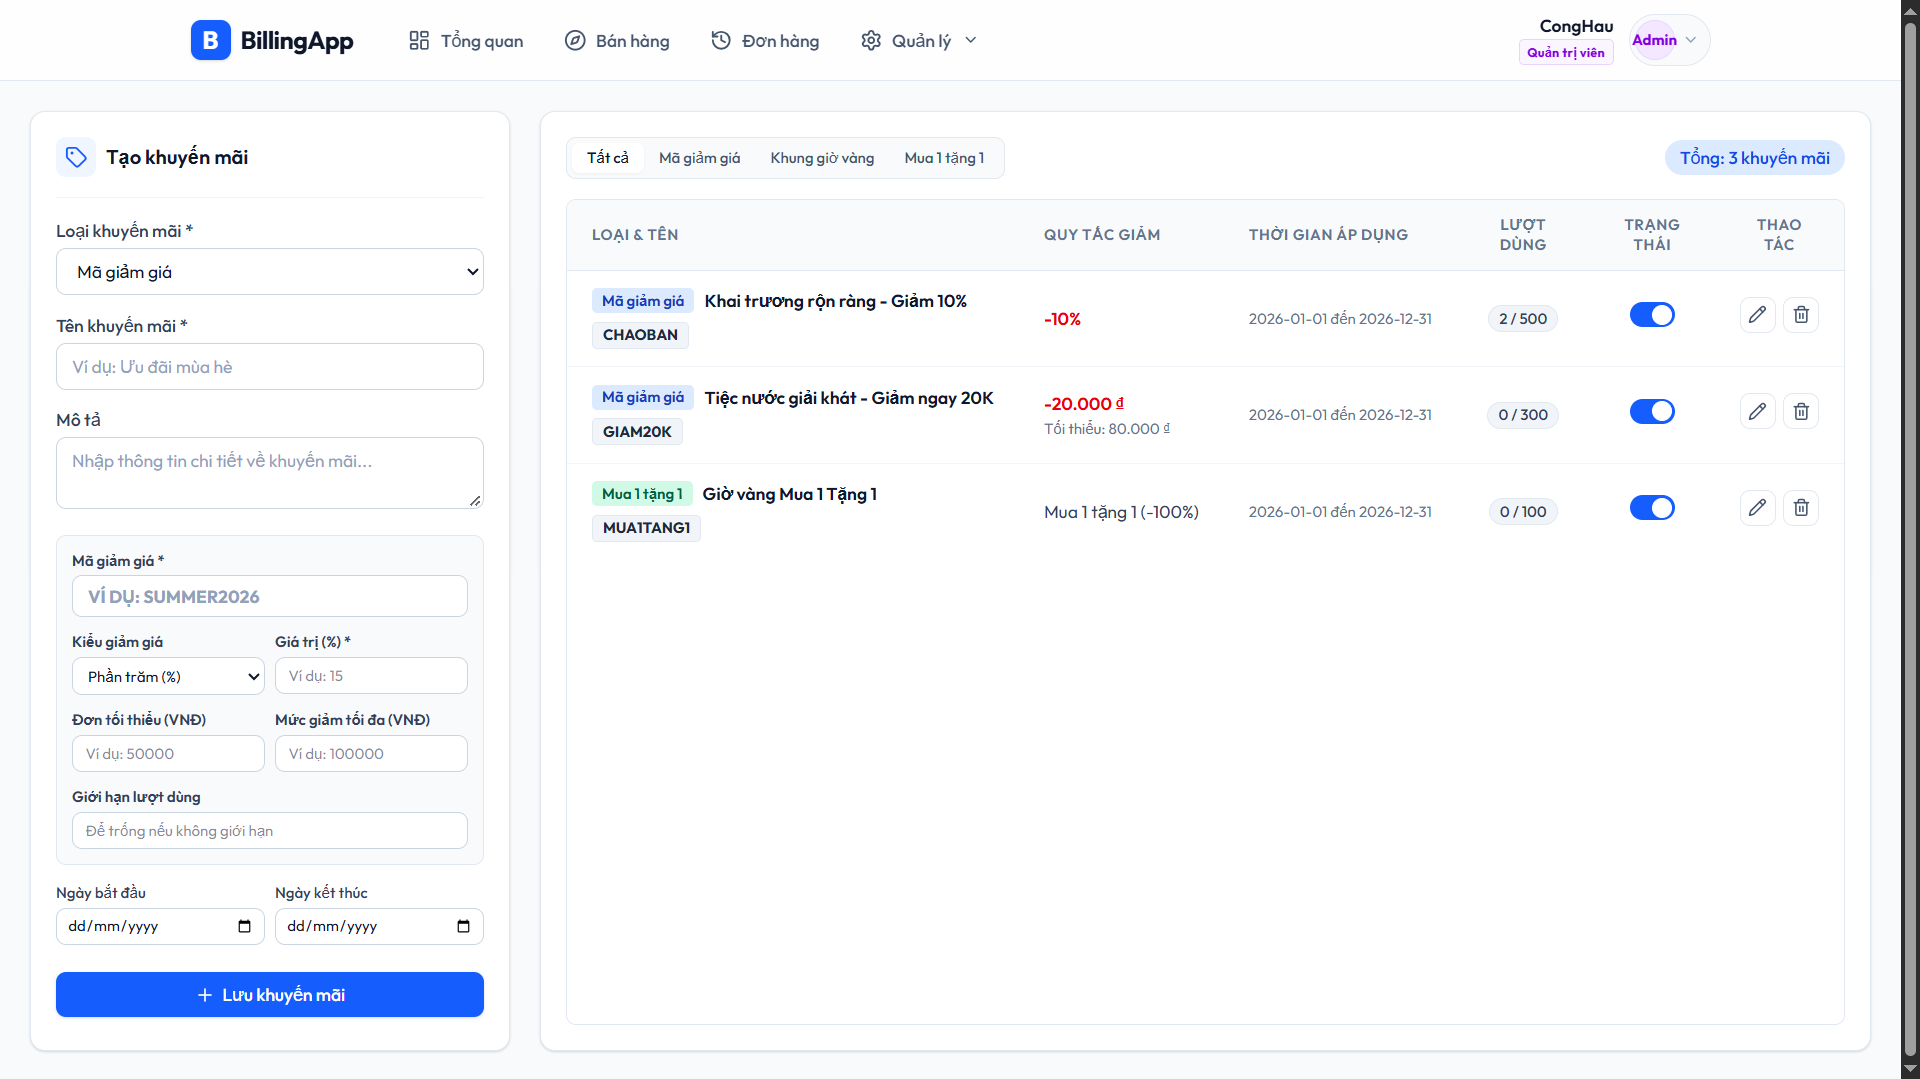
\includegraphics[width=0.92\textwidth]{images/ui_manage_promotions.png}
}{
    \fbox{\parbox{0.9\textwidth}{\centering \vspace{12mm}
    \textbf{[HÌNH 3.12: GIAO DIỆN QUẢN LÝ CHƯƠNG TRÌNH KHUYẾN MÃI (PROMOTIONS)]}\\
    \textit{(Vị trí ảnh chụp: report/images/ui\_manage\_promotions.png)}\\
    \vspace{12mm}}}
}
\caption{Giao diện Quản lý Chương trình Khuyến mãi đa quy tắc}
\label{fig:ui_manage_promotions}
\end{figure}

\begin{figure}[H]
\centering
\IfFileExists{images/ui_manage_customers.png}{
    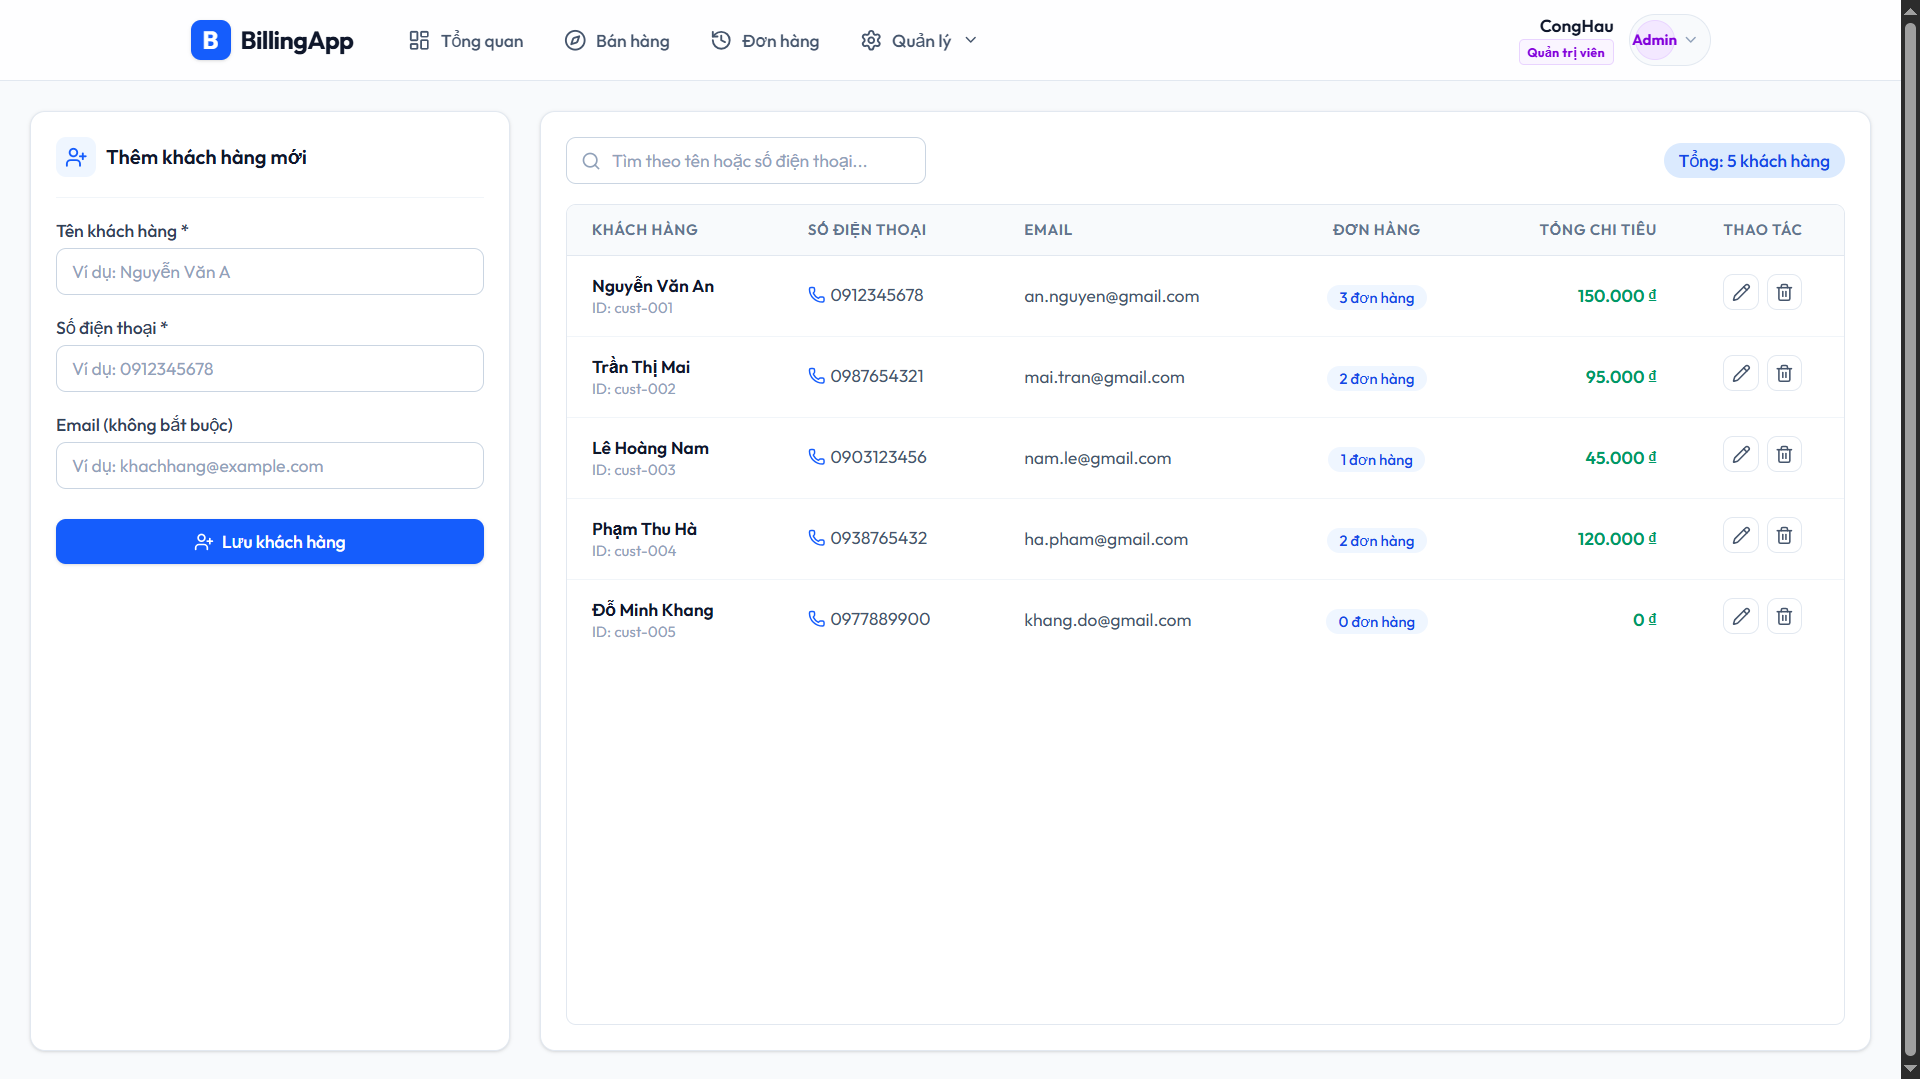
\includegraphics[width=0.92\textwidth]{images/ui_manage_customers.png}
}{
    \fbox{\parbox{0.9\textwidth}{\centering \vspace{12mm}
    \textbf{[HÌNH 3.13: GIAO DIỆN QUẢN LÝ DANH BẠ KHÁCH HÀNG THÂN THIẾT CRM]}\\
    \textit{(Vị trí ảnh chụp: report/images/ui\_manage\_customers.png)}\\
    \vspace{12mm}}}
}
\caption{Giao diện Quản lý Khách hàng thân thiết CRM}
\label{fig:ui_manage_customers}
\end{figure}

\begin{figure}[H]
\centering
\IfFileExists{images/ui_manage_users.png}{
    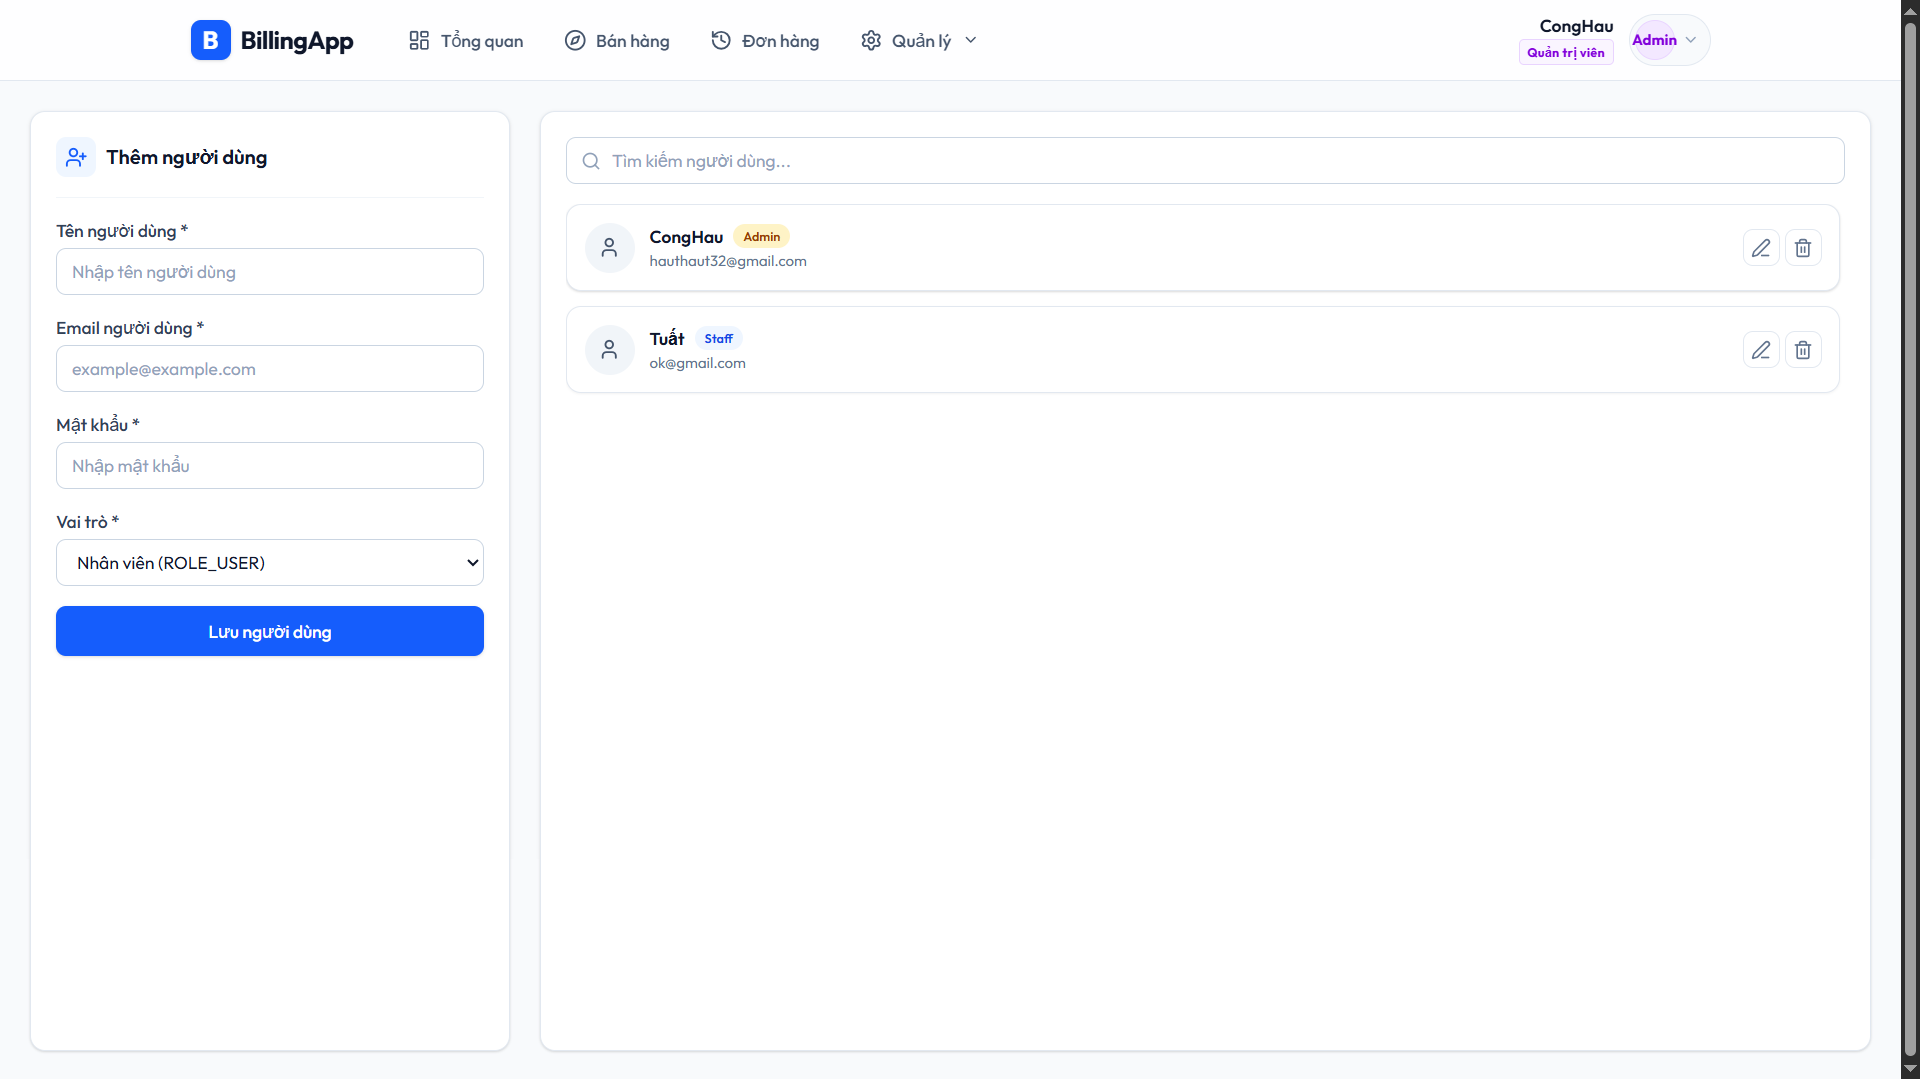
\includegraphics[width=0.92\textwidth]{images/ui_manage_users.png}
}{
    \fbox{\parbox{0.9\textwidth}{\centering \vspace{12mm}
    \textbf{[HÌNH 3.14: GIAO DIỆN QUẢN TRỊ NGƯỜI DÙNG VÀ PHÂN QUYỀN RBAC]}\\
    \textit{(Vị trí ảnh chụp: report/images/ui\_manage\_users.png)}\\
    \vspace{12mm}}}
}
\caption{Giao diện Quản trị Người dùng và Phân quyền RBAC}
\label{fig:ui_manage_users}
\end{figure}

\begin{figure}[H]
\centering
\IfFileExists{images/ui_activity_logs.png}{
    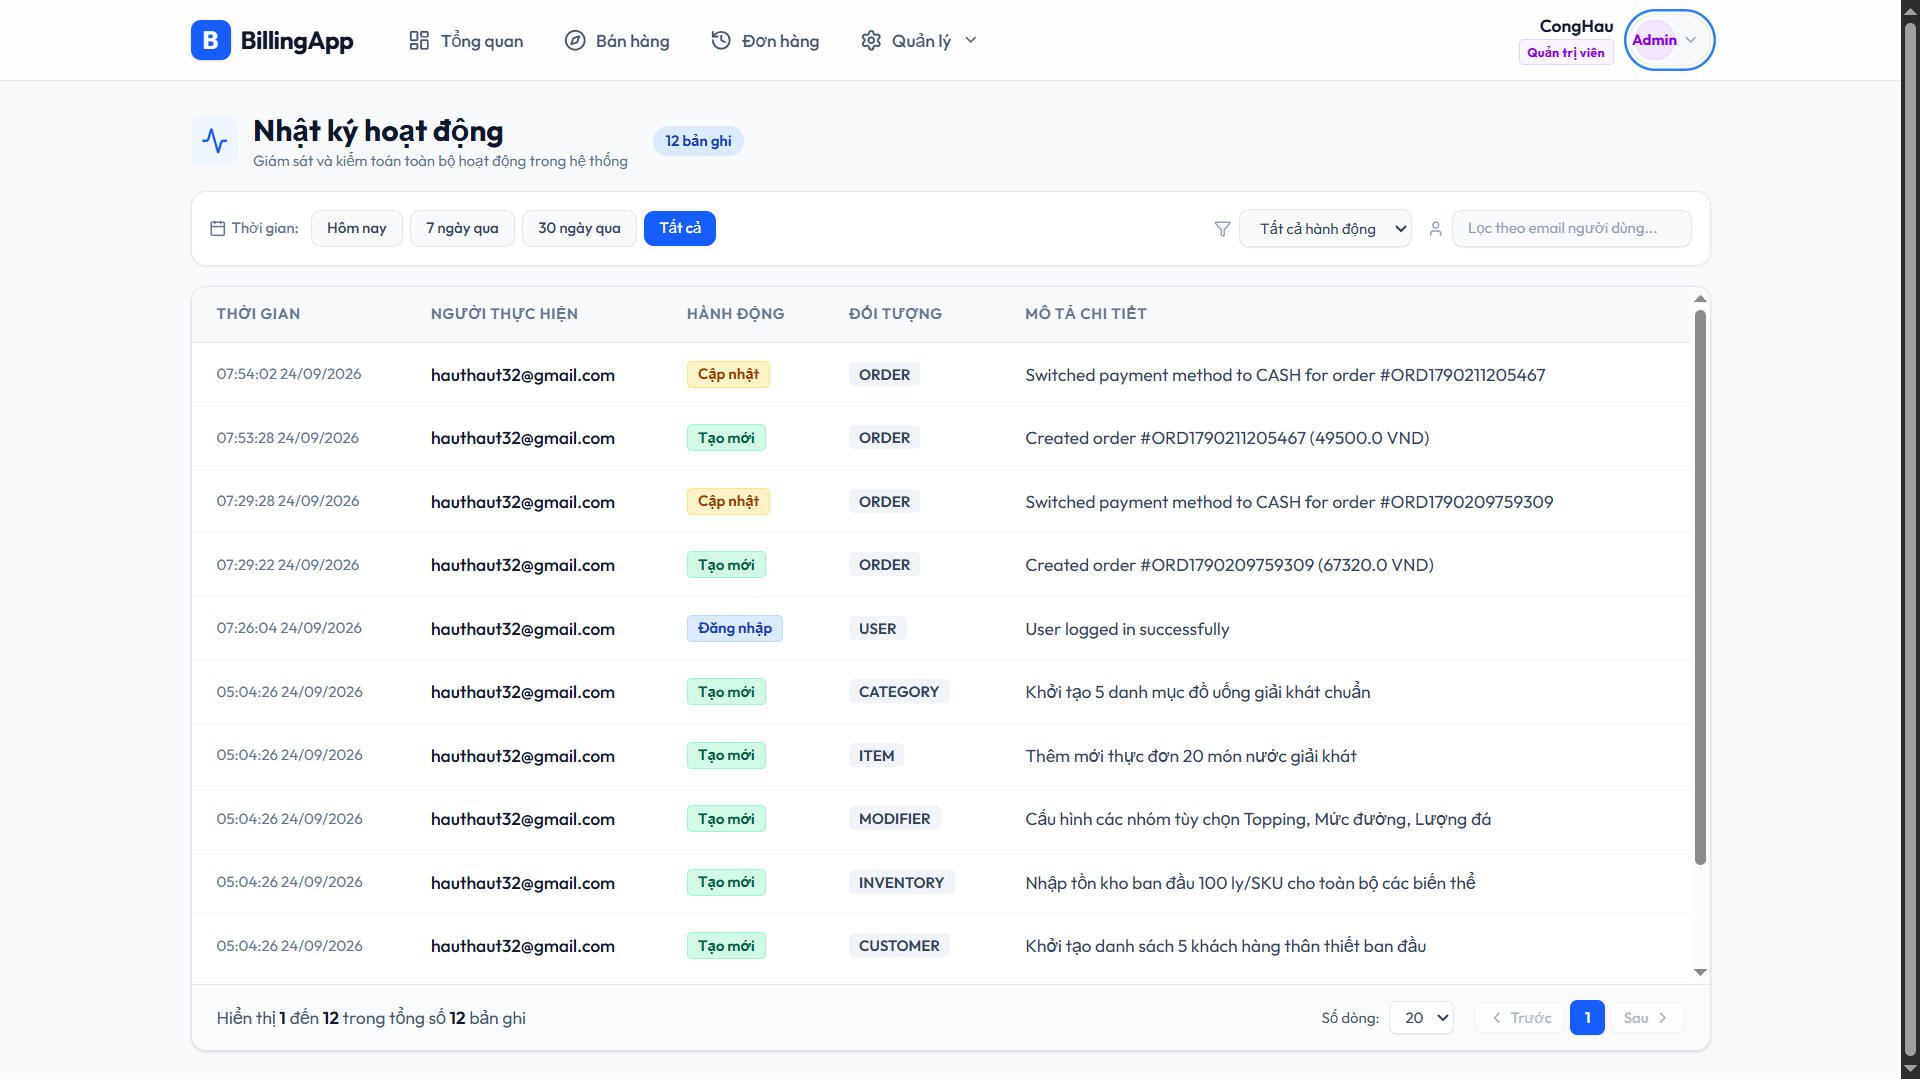
\includegraphics[width=0.92\textwidth]{images/ui_activity_logs.png}
}{
    \fbox{\parbox{0.9\textwidth}{\centering \vspace{12mm}
    \textbf{[HÌNH 3.15: GIAO DIỆN NHẬT KÝ KIỂM TOÁN HOẠT ĐỘNG (ACTIVITY LOGS)]}\\
    \textit{(Vị trí ảnh chụp: report/images/ui\_activity\_logs.png)}\\
    \vspace{12mm}}}
}
\caption{Giao diện Nhật ký Kiểm toán Hoạt động hệ thống (Activity Logs)}
\label{fig:ui_activity_logs}
\end{figure}


% ==============================================================================
\section{Trích xuất thuật toán và xử lý nghiệp vụ cốt lõi}
\label{sec:thuat_toan_cot_loi}

Dưới đây là 5 đoạn mã nguồn trích xuất từ các thành phần xử lý trọng yếu nhất trong hệ thống Back-end, minh chứng cho tính chuẩn mực và chiều sâu kỹ thuật của dự án.

\subsection{Thuật toán 1: Trừ kho theo cơ chế Sổ cái và Giao dịch bù trừ khi hủy đơn}
Đoạn mã trích xuất từ \texttt{OrderServiceImpl.java} thể hiện việc ghi nhận giao dịch xuất kho \texttt{OUT} có số lượng âm khi tạo đơn hàng và cập nhật lại trường tồn kho đệm \texttt{cachedStockQuantity}:

\begin{lstlisting}[language=Java, caption={Thuật toán trừ kho sổ cái khi tạo đơn hàng mới}]
// Trừ kho thông qua sổ cái giao dịch (Inventory Ledger OUT)
for (OrderItemEntity item : newOrder.getItems()) {
    VariantEntity variant = null;
    if (item.getVariantId() != null && !item.getVariantId().trim().isEmpty()) {
        variant = variantRepository.findByVariantId(item.getVariantId()).orElse(null);
    }

    if (variant != null) {
        int soldQuantity = item.getQuantity() != null ? item.getQuantity() : 1;
        InventoryTransactionEntity transaction = InventoryTransactionEntity.builder()
                .transactionId(UUID.randomUUID().toString())
                .variant(variant)
                .transactionType(TransactionType.OUT)
                .quantity(-Math.abs(soldQuantity)) // Số lượng âm biểu thị xuất kho bán lẻ
                .referenceId(newOrder.getOrderId())
                .note("POS Sale - Order " + newOrder.getOrderId())
                .build();
        inventoryTransactionRepository.saveAndFlush(transaction);

        // Tính toán lại tồn kho thực tế từ tổng các giao dịch và đồng bộ vào cache
        Integer updatedStock = inventoryTransactionRepository.calculateStockByVariantId(variant.getVariantId());
        variant.setCachedStockQuantity(updatedStock != null ? updatedStock : 0);
        variantRepository.save(variant);
    }
}
\end{lstlisting}

Đồng thời, khi đơn hàng chờ (\texttt{PENDING}) bị hủy, phương thức \texttt{compensatePendingOrder} tự động kích hoạt giao dịch bù trừ \texttt{IN} để hoàn kho chính xác:

\begin{lstlisting}[language=Java, caption={Cơ chế giao dịch bù trừ (Compensating Transaction) khi hủy đơn}]
private void compensatePendingOrder(OrderEntity order, String referenceId, String reason) {
    // 1. Giao dịch bù trừ kho (Compensating Ledger Transaction IN)
    if (order.getItems() != null) {
        for (OrderItemEntity item : order.getItems()) {
            VariantEntity variant = variantRepository.findByVariantId(item.getVariantId()).orElse(null);
            if (variant != null) {
                int returnQty = Math.abs(item.getQuantity() != null ? item.getQuantity() : 1);
                InventoryTransactionEntity revertTx = InventoryTransactionEntity.builder()
                        .transactionId(UUID.randomUUID().toString())
                        .variant(variant)
                        .transactionType(TransactionType.IN)
                        .quantity(returnQty) // Nhập hoàn lại kho
                        .referenceId(referenceId)
                        .note("Hoàn kho: " + reason)
                        .build();
                inventoryTransactionRepository.saveAndFlush(revertTx);

                Integer updatedStock = inventoryTransactionRepository.calculateStockByVariantId(variant.getVariantId());
                variant.setCachedStockQuantity(updatedStock != null ? updatedStock : 0);
                variantRepository.save(variant);
            }
        }
    }
    // 2. Hoàn lại số lượt sử dụng voucher khuyến mãi
    if (order.getPromotionId() != null) {
        PromotionEntity promo = promotionRepository.findByPromotionId(order.getPromotionId()).orElse(null);
        if (promo != null && promo.getTimesUsed() != null && promo.getTimesUsed() > 0) {
            promo.setTimesUsed(promo.getTimesUsed() - 1);
            promotionRepository.save(promo);
        }
    }
}
\end{lstlisting}

\subsection{Thuật toán 2: Tính toán tổng tiền, VAT 10\% và chiết khấu khuyến mãi}
Toàn bộ quá trình tính toán tiền tệ được thực hiện phía máy chủ nhằm đảm bảo tính bảo mật và chống gian lận thay đổi giá từ phía client:

\begin{lstlisting}[language=Java, caption={Thuật toán tính toán tài chính và thuế VAT phía Server}]
// 1. Tính tổng tiền hàng gốc trước thuế và giảm giá (Subtotal)
BigDecimal subtotal = BigDecimal.ZERO;
for (EvaluationCartItem item : request.getCartItems()) {
    BigDecimal itemPrice = item.getPrice() != null ? item.getPrice() : BigDecimal.ZERO;
    BigDecimal itemQuantity = BigDecimal.valueOf(item.getQuantity() != null ? item.getQuantity() : 1);
    subtotal = subtotal.add(itemPrice.multiply(itemQuantity));
}

// 2. Xác định chiết khấu khuyến mãi tối ưu (Discount Amount)
BigDecimal discountAmount = bestCandidate != null ? bestCandidate.getDiscountAmount() : BigDecimal.ZERO;

// 3. Tính tiền hàng chịu thuế sau giảm giá
BigDecimal taxableAmount = subtotal.subtract(discountAmount).max(BigDecimal.ZERO);

// 4. Tính thuế giá trị gia tăng VAT 10%
BigDecimal tax = taxableAmount.multiply(BigDecimal.valueOf(0.10)).setScale(2, RoundingMode.HALF_UP);

// 5. Tính tổng thanh toán cuối cùng (Grand Total)
BigDecimal grandTotal = taxableAmount.add(tax).setScale(2, RoundingMode.HALF_UP);
\end{lstlisting}

\subsection{Thuật toán 3: Bộ lọc xác thực và phân giải quyền hạn (JwtRequestFilter)}
Bộ lọc \texttt{JwtRequestFilter} kế thừa \texttt{OncePerRequestFilter} thực hiện kiểm tra tính hợp lệ của JWT Access Token trên mỗi yêu cầu gửi tới:

\begin{lstlisting}[language=Java, caption={Bộ lọc an ninh JwtRequestFilter}]
@Override
protected void doFilterInternal(HttpServletRequest request, HttpServletResponse response, FilterChain filterChain) 
        throws ServletException, IOException {
    final String authorizationHeader = request.getHeader("Authorization");
    String email = null;
    String jwt = null;

    try {
        if (authorizationHeader != null && authorizationHeader.startsWith("Bearer ")) {
            jwt = authorizationHeader.substring(7);
            email = jwtUtil.extractUsername(jwt);
        }

        if (email != null && SecurityContextHolder.getContext().getAuthentication() == null) {
            UserDetails userDetails = userDetailsService.loadUserByUsername(email);
            if (jwtUtil.validateToken(jwt, userDetails)) {
                UsernamePasswordAuthenticationToken authenticationToken =
                        new UsernamePasswordAuthenticationToken(userDetails, null, userDetails.getAuthorities());
                authenticationToken.setDetails(new WebAuthenticationDetailsSource().buildDetails(request));
                SecurityContextHolder.getContext().setAuthentication(authenticationToken);
            }
        }
    } catch (JwtException | IllegalArgumentException exception) {
        // Xóa sạch ngữ cảnh an ninh khi token không hợp lệ hoặc hết hạn -> Spring Security trả 401
        SecurityContextHolder.clearContext();
    }
    filterChain.doFilter(request, response);
}
\end{lstlisting}

\subsection{Thuật toán 4: Bộ máy đánh giá khuyến mãi tối ưu không xếp chồng (No Stacking)}
Thuật toán so sánh toàn bộ các chương trình ưu đãi hiện hành và chọn ra duy nhất một chương trình có mức chiết khấu cao nhất (trích từ \texttt{PromotionServiceImpl.java}):

\begin{lstlisting}[language=Java, caption={Thuật toán lựa chọn khuyến mãi tối ưu nhất}]
// So sánh và chọn khuyến mãi có mức giảm cao nhất (No Stacking - ADR-0003)
PromotionCandidateDto bestCandidate = null;
for (PromotionCandidateDto candidate : candidates) {
    if (bestCandidate == null) {
        bestCandidate = candidate;
    } else if (candidate.getDiscountAmount().compareTo(bestCandidate.getDiscountAmount()) > 0) {
        bestCandidate = candidate;
    }
}

// Nếu có mã Coupon người dùng nhập, so sánh với khuyến mãi tự động tốt nhất
if (couponCandidate != null) {
    if (bestCandidate == null || couponCandidate.getDiscountAmount().compareTo(bestCandidate.getDiscountAmount()) >= 0) {
        bestCandidate = couponCandidate;
    }
}
\end{lstlisting}

\subsection{Thuật toán 5: Xử lý Webhook PayOS xác thực chữ ký số HMAC-SHA256}
Đoạn mã tiếp nhận Webhook từ cổng PayOS, thẩm định chữ ký điện tử để cập nhật trạng thái đơn hàng (trích từ \texttt{PaymentWebhookController.java}):

\begin{lstlisting}[language=Java, caption={Bộ điều khiển tiếp nhận và xác thực chữ ký Webhook PayOS}]
@PostMapping("/webhook")
public ResponseEntity<?> handleWebhook(@RequestBody Webhook webhookBody) {
    try {
        // PayOS SDK tự động kiểm tra chữ ký điện tử dựa trên checksumKey
        WebhookData data = payOS.webhooks().verify(webhookBody);

        // Kiểm tra mã giao dịch thành công ("00")
        if ("00".equals(data.getCode())) {
            Long orderCode = data.getOrderCode();
            OrderEntity order = orderRepository.findById(orderCode)
                    .orElseThrow(() -> new RuntimeException("Không tìm thấy đơn hàng #" + orderCode));

            // Cập nhật trạng thái thanh toán sang COMPLETED
            if (order.getPaymentDetails() != null) {
                order.getPaymentDetails().setStatus(PaymentDetails.PaymentStatus.COMPLETED);
            }
            orderRepository.save(order);
            return ResponseEntity.ok("success");
        }
        return ResponseEntity.badRequest().body("Giao dịch không thành công");
    } catch (PayOSException e) {
        // Trả lỗi 400 nếu chữ ký không khớp (dấu hiệu giả mạo Webhook)
        return ResponseEntity.badRequest().body("Webhook verify failed: " + e.getMessage());
    }
}
\end{lstlisting}

% ==============================================================================
% MỤC 3.5: MA TRẬN KIỂM THỬ VÀ ĐÁNH GIÁ CHẤT LƯỢNG HỆ THỐNG
% ==============================================================================
% ==============================================================================
% 03_CHAPTER3_PART2_TESTING.TEX - KIỂM THỬ HỆ THỐNG VÀ ĐÁNH GIÁ KẾT QUẢ
% ==============================================================================

\section{Kiểm thử hệ thống (System Testing)}
\label{sec:kiem_thu_he_thong}

\subsection{Mục tiêu và phương pháp kiểm thử}
Kiểm thử phần mềm là giai đoạn then chốt nhằm phát hiện sớm các khiếm khuyết kỹ thuật, thẩm định tính chính xác của các quy tắc nghiệp vụ và đo lường độ tin cậy của hệ thống trước khi đưa vào vận hành thực tế tại điểm bán. Các mục tiêu kiểm thử bao gồm:
\begin{enumerate}[label=\arabic*., leftmargin=1.5cm]
    \item \textbf{Thẩm định tính đúng đắn về chức năng (Functional Verification):} Đảm bảo mọi tính năng từ đăng nhập, bán hàng, tính thuế VAT, đánh giá khuyến mãi đến thanh toán trực tuyến đều hoạt động đúng theo các ca sử dụng đã đặc tả tại Chương 2.
    \item \textbf{Đảm bảo tính toàn vẹn tài chính và kế toán:} Kiểm tra nghiêm ngặt việc cấm xóa đơn hàng đã hoàn tất (\texttt{COMPLETED}), kiểm tra tính chính xác của giao dịch bù trừ hoàn kho (\texttt{IN}) khi hủy đơn chờ.
    \item \textbf{Kiểm tra tính an toàn thông tin (Security Verification):} Kiểm định cơ chế kiểm soát truy cập theo vai trò (RBAC), khả năng chống tấn công phát lại mã phiên (Replay Attack) của cơ chế Token Rotation, và tính toàn vẹn của chữ ký số Webhook PayOS.
    \item \textbf{Đo lường hiệu năng phản hồi (Performance Verification):} Xác nhận thời gian phản hồi tại quầy thu ngân đạt tiêu chuẩn dưới $1$ giây đối với mọi thao tác bán hàng.
\end{enumerate}

Phương pháp kiểm thử chủ đạo được áp dụng là \textbf{Kiểm thử Hộp đen (Black-box Testing)} kết hợp cùng \textbf{Kiểm thử Tích hợp (Integration Testing)} đa tầng giữa ứng dụng ReactJS SPA, máy chủ Spring Boot API và các dịch vụ đám mây bên thứ ba (PayOS, AWS S3).

\subsection{Môi trường và bộ dữ liệu kiểm thử}
Hệ thống được kiểm thử trên môi trường phần cứng và dữ liệu chuẩn:
\begin{itemize}[leftmargin=1.5cm]
    \item \textbf{Thiết bị thử nghiệm máy khách (Client):} Máy tính xách tay CPU Intel Core i7, 16GB RAM, kết nối mạng LAN/Wi-Fi 5GHz; màn hình độ phân giải Full HD ($1920\times 1080$), trình duyệt Google Chrome phiên bản 128. Kết nối máy in nhiệt Xprinter chuẩn 80mm qua cổng USB.
    \item \textbf{Môi trường máy chủ (Server):} Hệ điều hành Windows 11 / Docker Desktop Linux Container, máy chủ ảo hóa Java 25 Runtime, MySQL Server 8.0 với InnoDB Engine.
    \item \textbf{Bộ dữ liệu thử nghiệm chuẩn (Test Dataset):}
    \begin{itemize}
        \item 5 danh mục hàng hóa (Cà phê, Trà sữa, Nước ép, Bánh ngọt, Đồ ăn vặt).
        \item 30 sản phẩm cơ sở với 65 biến thể SKU (phân loại Size S/M/L, Màu sắc).
        \item 4 nhóm tùy chọn Modifier (Topping, Mức đường, Mức đá, Kem Cheese).
        \item 5 chương trình khuyến mãi thử nghiệm (1 Happy Hour khung giờ vàng 14h-17h, 1 BOGO mua Trà sữa size L tặng size M, 2 mã Coupon giảm 20\% và 50.000đ).
        \item 15 hồ sơ khách hàng thân thiết CRM với các hạn mức chi tiêu tích lũy khác nhau.
        \item 3 tài khoản người dùng: 1 Quản trị viên (\texttt{admin@billing.com}) và 2 Thu ngân (\texttt{staff1@billing.com}, \texttt{staff2@billing.com}).
    \end{itemize}
\end{itemize}

\subsection{Ma trận kịch bản kiểm thử chi tiết (Test Cases Matrix)}
Dưới đây là bảng ma trận 15 ca kiểm thử đại diện cho các luồng nghiệp vụ cốt lõi và các tình huống ngoại lệ của hệ thống POS (Bảng \ref{tab:test_cases_matrix}).

\begin{longtable}{|c|p{3.2cm}|p{3.8cm}|p{4.2cm}|c|}
\caption{Ma trận kịch bản kiểm thử chức năng và an ninh hệ thống} \label{tab:test_cases_matrix} \\
\hline
\textbf{Mã ca} & \textbf{Tên ca kiểm thử} & \textbf{Dữ liệu \& Các bước thực hiện} & \textbf{Kết quả mong đợi} & \textbf{Kết quả} \\ \hline
\endfirsthead
\hline
\textbf{Mã ca} & \textbf{Tên ca kiểm thử} & \textbf{Dữ liệu \& Các bước thực hiện} & \textbf{Kết quả mong đợi} & \textbf{Kết quả} \\ \hline
\endhead
\hline
\endfoot
\hline
\endlastfoot

\textbf{TC01} & Đăng nhập với mật khẩu không chính xác & Nhập email: \texttt{staff1@billing.com}, mật khẩu: \texttt{WrongPass123!}, nhấn ''Đăng nhập''. & Trả mã HTTP 401. Giao diện hiển thị toast lỗi tiếng Việt: ''Email hoặc mật khẩu không chính xác''. Không cấp token. & \textbf{PASS} \\ \hline

\textbf{TC02} & Đăng nhập thành công với vai trò Thu ngân & Nhập email: \texttt{staff1@billing.com}, mật khẩu đúng, nhấn ''Đăng nhập''. & Trả mã HTTP 200. Access Token lưu trong RAM. Cookie \texttt{refreshToken} (HttpOnly) được tạo. Tự động điều hướng vào \texttt{/explore}. & \textbf{PASS} \\ \hline

\textbf{TC03} & Kiểm soát phân quyền RBAC (\texttt{AdminRoute}) & Tài khoản Thu ngân cố tình truy cập thủ công vào URL quản trị: \texttt{/users} hoặc \texttt{/promotions}. & Hệ thống phát hiện vai trò không phải \texttt{ROLE\_ADMIN}, hiển thị toast cảnh báo từ chối truy cập và tự động đẩy về \texttt{/dashboard}. & \textbf{PASS} \\ \hline

\textbf{TC04} & Tìm kiếm sản phẩm thông minh (Debounce) & Tại thanh tìm kiếm quầy POS, gõ chuỗi ký tự ''tra sua''. & Sau khoảng nghỉ $300$ms, danh sách sản phẩm lọc đúng các mặt hàng trà sữa. Tốc độ lọc mượt mà, không giật lag. & \textbf{PASS} \\ \hline

\textbf{TC05} & Chọn Biến thể SKU và tùy chọn Modifier & Chọn Trà sữa Oolong, mở modal: chọn Size L (+$5.000$đ), chọn Trân châu trắng (+$10.000$đ), chọn 50\% đường. Nhấn thêm giỏ. & Mặt hàng được đưa vào giỏ với đơn giá đã cộng chính xác phụ thu ($55.000$đ). Hiển thị chi tiết lựa chọn kèm theo. & \textbf{PASS} \\ \hline

\textbf{TC06} & Nhận diện khách hàng thân thiết CRM & Nhập số điện thoại \texttt{0987654321} vào ô tìm kiếm khách hàng tại giỏ hàng. & Hệ thống tìm kiếm theo thời gian thực, hiển thị đúng họ tên khách hàng, số điểm tích lũy và tổng chi tiêu trước đó. & \textbf{PASS} \\ \hline

\textbf{TC07} & Tự động áp dụng khuyến mãi Happy Hour & Đặt đơn hàng trị giá $120.000$đ trong khung giờ 14h00 - 17h00 (chương trình giảm 15\% cho đơn từ $100$k). & Hệ thống tự động tính chiết khấu $18.000$đ. Tiền hàng chịu thuế giảm còn $102.000$đ. Thuế VAT 10\% là $10.200$đ. Tổng tiền là $112.200$đ. & \textbf{PASS} \\ \hline

\textbf{TC08} & Áp dụng mã Coupon hợp lệ và hết hạn & 1. Nhập mã \texttt{SALE20} hợp lệ $\rightarrow$ được giảm 20\%. \newline 2. Nhập mã \texttt{HETHAN50} đã hết hạn $\rightarrow$ nhấn áp dụng. & 1. Áp dụng mã thành công, hiển thị chiết khấu. \newline 2. Báo lỗi: ''Mã giảm giá đã hết hạn sử dụng'', giỏ hàng giữ nguyên giá trị gốc. & \textbf{PASS} \\ \hline

\textbf{TC09} & Thanh toán Tiền mặt và In hóa đơn nhiệt 80mm & Tổng đơn $112.200$đ. Thu ngân chọn Tiền mặt, bấm nút gợi ý nhận $200.000$đ từ khách. Nhấn ''Hoàn tất''. & Hệ thống tính tiền thừa thối lại: $87.800$đ. Mở popup in bill nhiệt 80mm với đầy đủ thông tin, kích hoạt lệnh in trình duyệt. & \textbf{PASS} \\ \hline

\textbf{TC10} & Trừ kho sổ cái khi tạo đơn hàng mới & Đơn hàng bán 2 cốc Trà sữa Oolong Size L (kho hiện có 50). Hoàn tất thanh toán. & Bảng sổ cái ghi nhận 1 giao dịch \texttt{OUT} với số lượng là $-2$. Trường \texttt{cachedStockQuantity} của biến thể giảm xuống 48. & \textbf{PASS} \\ \hline

\textbf{TC11} & Thanh toán trực tuyến VietQR PayOS & Chọn phương thức \texttt{PAYOS}. Mở popup QR. Khách quét mã chuyển tiền qua App Ngân hàng. & PayOS gửi Webhook xác thực SHA-256 Checksum hợp lệ. Đơn chuyển \texttt{COMPLETED}. Màn hình POS tự động nhận và mở bill. & \textbf{PASS} \\ \hline

\textbf{TC12} & Chuyển đổi phương thức thanh toán (\textit{Switch to Cash}) & Khách chọn PayOS nhưng app ngân hàng bảo trì. Thu ngân nhấn ''Chuyển sang tiền mặt''. & Đơn hàng chuyển sang \texttt{CASH} \texttt{COMPLETED}. Link PayOS bị hủy từ xa. Hệ thống hoàn tất đơn mà không nhân đôi xuất kho. & \textbf{PASS} \\ \hline

\textbf{TC13} & Hủy đơn hàng PENDING và Bù trừ kho tự động & Đơn hàng chờ chuyển khoản bị khách hủy. Thu ngân nhấn nút ''Hủy đơn hàng'' tại màn hình Lịch sử đơn. & Đơn chuyển \texttt{CANCELLED}. Sổ cái tự động tạo giao dịch \texttt{IN} (+2) hoàn trả kho. Hoàn lại 1 lượt dùng voucher. Giảm trừ CRM. & \textbf{PASS} \\ \hline

\textbf{TC14} & Chống xóa đơn hàng đã hoàn tất (\texttt{COMPLETED}) & Thu ngân hoặc hacker cố tình gửi request \texttt{DELETE /api/v1.0/orders/\{id\}} với đơn hàng đã thanh toán. & Máy chủ từ chối với mã lỗi 400 Bad Request: ''Nghiêm cấm xóa đơn hàng đã hoàn tất''. Bảo vệ nguyên vẹn dữ liệu tài chính. & \textbf{PASS} \\ \hline

\textbf{TC15} & Ngăn chặn Replay Attack với Refresh Token (ADR-0007) & Kẻ gian đánh cắp và cố tình sử dụng lại một Refresh Token cũ đã từng được xoay vòng trước đó. & Máy chủ phát hiện token đã thu hồi (\texttt{revokedAt} khác null), lập tức vô hiệu hóa toàn bộ nhóm \texttt{familyId}, buộc đăng nhập lại. & \textbf{PASS} \\
\end{longtable}

\subsection{Đánh giá và tổng kết kết quả kiểm thử}
Kết quả thực nghiệm trên toàn bộ 15 kịch bản kiểm thử trọng yếu (Bảng \ref{tab:test_summary}) khẳng định:
\begin{itemize}[leftmargin=1.5cm]
    \item \textbf{Độ tin cậy chức năng đạt 100\%:} Toàn bộ các ca kiểm thử nghiệp vụ bán hàng, quản lý biến thể, tính toán tài chính và tích hợp cổng thanh toán VietQR PayOS đều đạt kết quả mong đợi (15/15 Pass).
    \item \textbf{Hiệu năng đáp ứng vượt trội:} Thời gian xử lý trung bình của máy chủ API Spring Boot cho các tác vụ tạo đơn hàng và trừ kho sổ cái chỉ dao động trong khoảng $120$ms – $250$ms; thời gian cập nhật giao diện Front-end đạt dưới $30$ms, đáp ứng hoàn hảo tiêu chí phản hồi dưới $1$ giây đặt ra ban đầu.
    \item \textbf{Tính toàn vẹn kế toán và an toàn dữ liệu được bảo vệ tuyệt đối:} Quy trình bù trừ giao dịch kho khi hủy đơn (\texttt{compensatePendingOrder}) và cơ chế ngăn chặn xóa đơn đã hoàn tất đảm bảo số liệu doanh thu và tồn kho của cửa hàng luôn minh bạch và chính xác tuyệt đối.
\end{itemize}

\begin{table}[htbp]
\centering
\caption{Bảng tổng hợp kết quả kiểm thử hệ thống}
\label{tab:test_summary}
\vspace{2mm}
\begin{tabularx}{\textwidth}{|p{4.5cm}|c|c|c|X|}
\hline
\textbf{Nhóm kiểm thử} & \textbf{Tổng số ca} & \textbf{Đạt (Pass)} & \textbf{Không đạt} & \textbf{Tỷ lệ thành công} \\ \hline
Xác thực, Phân quyền \& Bảo mật & 4 & 4 & 0 & 100\% \\ \hline
Nghiệp vụ Bán hàng POS \& CRM & 4 & 4 & 0 & 100\% \\ \hline
Tính toán Khuyến mãi \& Thuế VAT & 2 & 2 & 0 & 100\% \\ \hline
Thanh toán PayOS \& Chuyển đổi & 2 & 2 & 0 & 100\% \\ \hline
Quản lý Kho sổ cái \& Toàn vẹn & 3 & 3 & 0 & 100\% \\ \hline
\textbf{TỔNG CỘNG} & \textbf{15} & \textbf{15} & \textbf{0} & \textbf{100\% (ĐẠT CHUẨN)} \\ \hline
\end{tabularx}
\end{table}

% ==============================================================================
\section{Tổng kết chương 3}
Chương 3 đã hoàn thành xuất sắc việc trình bày quá trình cài đặt, hiện thực hóa và kiểm thử thực nghiệm toàn bộ hệ thống POS Quản lý bán hàng. Các giải pháp kiến trúc đã được hiện thực hóa sống động qua 11 màn hình giao diện thực tế của cả phân hệ Thu ngân và Quản trị, từ giao diện bán hàng nhanh, popup biến thể SKU, thanh toán VietQR động đến mẫu in nhiệt 80mm. Năm thuật toán cốt lõi về quản lý kho theo sổ cái, tính toán tài chính phía server, bộ lọc JWT, đánh giá khuyến mãi no-stacking và xác thực chữ ký số Webhook PayOS đã được phân tích minh bạch qua các đoạn mã nguồn Java thực tế. Cuối cùng, ma trận 15 kịch bản kiểm thử toàn diện đã chứng minh tính ổn định, độ bảo mật cao và hiệu năng phản hồi nhanh chóng của hệ thống, khẳng định tính khả thi và giá trị ứng dụng thực tiễn cao của đề tài.


